\documentclass[
  paper=a4, % DIN-A4-Format
  11pt, % Schriftgröße
  bibliography=totoc, % Bibliografie automatisch im Inhaltsverzeichnis generieren
  parskip=off, % Absatzabstand: off, half, full
  oneside, % einseitiges Layout
%  twoside, % zweiseitiges Layout
  article, % verwendet KOMA-Klasse scrartcl
%  longdoc=true,
  accentcolor=tud2b,
%  colorbacktitle, % Hintergrund des Titels einfärben
  colorback, % Hintergrund unter dem Titel einfärben
  type=bsc, % für Bachelorarbeit
]{tudthesis}

\usepackage[a-1b]{pdfx}

\usepackage[T1]{fontenc}
\usepackage[utf8]{inputenc} % korrekte Darstellung von Umlauten u. Sonderzeichen
\usepackage[stable]{footmisc} % mehr Optionen für Fußnoten
\usepackage{booktabs} % hübschere Tabellen als der LaTeX-Standard
\usepackage{multirow} % Create tabular cells spanning multiple rows
\usepackage{longtable} % große Tabellen, die sich über mehrere Seiten erstrecken
\usepackage{listings} % bietet Umgebung, um Programmiercode zu setzen inkl. Syntaxhighlighting
\usepackage{amsmath} % Setzen mathematischer Formeln
\usepackage{ellipsis} % korrigiert Aussehen von „…“
\usepackage{enumitem} % mehr Optionen für Aufzählungen
\usepackage[shortcuts]{extdash} % mehr Optionen für Worttrennung
\usepackage{setspace} % Zeilenabstände verändern: \singlespacing, \onehalfspacing oder \doublespacing
\usepackage{lipsum} % zur Erzeugung von Lorem-Ipsum-Blindtext
\usepackage[math]{blindtext} % zur Erzeugung von deutschem Blindtext
\usepackage{hyperref} % Verlinkungen im Dokument
\usepackage{csquotes}

% INFO %
% Das hyperref-Paket sollte möglichst als letztes geladen werden, darum steht es weiter hinten in der Präambel.
% Leider funktioniert hyperref nicht 100%-ig einwandfrei mit tudstyle; bei Problemen damit lieber aus dem Dokument entfernen!
% Einstellungen für hyperref
\hypersetup{%
    pdftitle=Motion R-CNN,
    pdfauthor=Simon Meister,
    pdfsubject=B.Sc. Thesis,
    unicode=true, % benötigt, damit Umlaute im pdftitle richtig dargestellt werden
    breaklinks=true
    %% colorlinks=true
    %% linkcolor=NavyBlue,
    %% urlcolor=NavyBlue,%Green4,
    %% citecolor=NavyBlue%DeepPink3
}

\usepackage[
    backend=biber, % biber ist das Standard-Backend für Biblatex. Für die Abwärtskompatibilität kann hier auch bibtex oder bibtex8 gewählt werden (siehe biblatex-Dokumentation)
    style=numeric, %numeric, authortitle, alphabetic etc.
    autocite=footnote, % Stil, der mit \autocite verwendet wird
    sorting=ynt, % Sortierung: nty = name title year, nyt = name year title u.a.
    sortcase=false,
    url=false,
    hyperref=auto,
    giveninits=true,
    maxbibnames=100
]{biblatex}

\renewbibmacro*{cite:seenote}{} % um zu verhindern, dass in Fußnoten automatisch "(wie Anm. xy)" eingefügt wird
\DeclareFieldFormat*{citetitle}{\mkbibemph{#1\isdot}} % zitierte Titel kursiv formatieren
\DeclareFieldFormat*{title}{\mkbibemph{#1\isdot}} % zitierte Titel kursiv formatieren

\addbibresource{bib.bib} % Hier Pfad zu deiner .bib-Datei hineinschreiben
\nocite{*} % Alle Einträge in der .bib-Datei im Literaturverzeichnis ausgeben, auch wenn sie nicht im Text zitiert werden. Gut zum Testen der .bib-Datei, sollte aber nicht generell verwendet werden. Stattdessen lieber gezielt Einträge mit Keywords ausgeben lassen (siehe \printbibliography in Zeile 224).


% INFO %
% Hier kannst du deine persönlichen Daten hineinschreiben und diese Variablen verwenden, damit du es nicht jedes Mal neu schreiben musst.
\newcommand*{\myname}{Simon Meister}
\newcommand*{\mytitlede}{Motion R-CNN: 3D-Bewegungsschätzung auf Instanzebene mit Regionsbasierten CNNs}
\newcommand*{\mytitleen}{Motion R-CNN: Instance-level 3D Motion Estimation with Region-based CNNs}
\newcommand*{\mymail}{\href{mailto:simon.meister@stud.tu-darmstadt.de}{simon.meister@stud.tu-darmstadt.de}}
\newcommand*{\myprof}{Prof. Stefan Roth, Ph.D.}
\newcommand*{\myinstitute}{Visual Inference Group}
\newcommand*{\myfaculty}{Fachbereich Informatik}

%%%%%%%%%%%%%%%%%%%%%%%%%%%%%%%%%%%%%%%%%%%%%%%%%%%%%%%%%%%%%%%%%%%%%%%%%%%%%%%%

\begin{document}
\parindent 0em % Erstzeileneinzug


\newcommand{\todo}[1]{\textbf{\textcolor{red}{#1}}}

% Titelei
\author{\myname}
\thesistitle{\mytitleen}{\mytitlede}
\birthplace{Erbach}
\date{21.11.2017}
\referee{\myprof}{M.Sc. Junhwa Hur}
\department{\myinstitute}
\group{\myfaculty}
\dateofexam{23.11.2017}{23.11.2017}
\makethesistitle

% Eigenständigkeitserklärung: muss nach \makethesistitle erscheinen, sonst wird sie als erste Seite des Dokuments gesetzt.
\affidavit[23.11.2017]{\myname}
%\affidavit{\myname}

\pagestyle{myheadings} % Seitenstil umschalten
\mymarkright{Version: \today} % Inhalt der Fußzeile


\begin{abstract}

% Many state of the art energy-minimization approaches to optical flow and scene
% flow estimation rely on a rigid scene model, where the scene is
% represented as an ensemble of distinct, rigidly moving components, a static
% background and a moving camera.
% By constraining the optimization problem with a physically sound scene model,
% these approaches enable state-of-the art motion estimation.

With the advent of deep learning methods, it has become popular to re-purpose
generic deep networks for classical computer vision problems involving
pixel-wise estimation.

Following this trend, many recent end-to-end deep learning approaches to optical
flow and scene flow predict full resolution flow fields with
a generic network for dense, pixel-wise prediction, thereby ignoring the
inherent structure of the underlying motion estimation problem and any physical
constraints within the scene.

We introduce a scalable end-to-end deep learning approach for dense motion estimation
that respects the structure of the scene as being composed of distinct objects,
thus combining the representation learning benefits and speed of end-to-end deep networks
with a physically plausible scene model inspired by slanted plane energy-minimization approaches to
scene flow.

Building on recent advanced in region-based convolutional networks (R-CNNs),
we integrate motion estimation with instance segmentation.
Given two consecutive frames from a monocular RGBD camera,
our resulting end-to-end deep network detects objects with accurate per-pixel
masks and estimates the 3D motion of each detected object between the frames.
By additionally estimating a global camera motion in the same network,
we compose a dense optical flow field based on instance-level and global motion
predictions. Our network is trained on the synthetic Virtual KITTI dataset,
which provides ground truth for all components of the system.

\end{abstract}

\renewcommand{\abstractname}{Zusammenfassung}
\begin{abstract}
\todo{german abstract}
\end{abstract}

\clearpage

%\pagenumbering{Roman} % Seitennummerierung auf römische Zahlen ändern

\setcounter{tocdepth}{3}
\tableofcontents
\setcounter{page}{1}
\clearpage

% Aktuelle Seitenzahl speichern, da Wechsel auf arabische Zahlen die Zählung zurücksetzt
%% \newcounter{savedromanpagenumber}
%% \setcounter{savedromanpagenumber}{\value{page}}
%\pagenumbering{arabic} % Arabische Seitenzahlen

\section{Introduction}
\parindent 2em
\onehalfspacing

\subsection{Motivation \& Goals}

For moving in the real world, it is generally desirable to know which objects exists
in the proximity of the moving agent,
where they are located relative to the agent,
and where they will be at some point in the future.
In many cases, it would be preferable to infer such information from video data
if technically feasible, as camera sensors are cheap and ubiquitous.

For example, in autonomous driving, it is crucial to not only know the position
of each obstacle, but to also know if and where the obstacle is moving,
and to use sensors that will not make the system too expensive for widespread use.

A promising approach for 3D scene understanding in situations like these are deep neural
networks, which have recently achieved breakthroughs in object detection, instance segmentation and classification
in still images and are more and more often being applied to video data.
A key benefit of end-to-end deep networks is that they can, in principle,
enable very fast inference on real time video data and generalize
over many training examples to resolve ambiguities inherent in image understanding
and motion estimation.

Thus, in this work, we aim to develop end-to-end deep networks which can, given
sequences of images, segment the image pixels into object instances and estimate
the location and 3D motion of each object instance relative to the camera.

\subsection{Technical outline}

Recently, SfM-Net \cite{SfmNet} introduced an end-to-end deep learning approach for predicting depth
and dense optical flow in monocular image sequences based on estimating the 3D motion of individual objects and the camera.
SfM-Net predicts a batch of binary full image masks specyfing the object memberships of individual pixels with a standard encoder-decoder
network for pixel-wise prediction. A fully connected network branching off the encoder predicts a 3D motion for each object.
However, due to the fixed number of objects masks, the system can only predict a small number of motions and
often fails to properly segment the pixels into the correct masks or assigns background pixels to object motions.

Thus, this approach is very unlikely to scale to dynamic scenes with a potentially
large number of diverse objects due to the inflexible nature of their instance segmentation technique.

A scalable approach to instance segmentation based on region-based convolutional networks
was recently introduced with Mask R-CNN \cite{MaskRCNN}, which inherits the ability to detect
a large number of objects from a large number of classes at once from Faster R-CNN
and predicts pixel-precise segmentation masks for each detected object.

We propose \emph{Motion R-CNN}, which combines the scalable instance segmentation capabilities of
Mask R-CNN with the end-to-end 3D motion estimation approach introduced with SfM-Net.
For this, we naturally integrate 3D motion prediction for individual objects into the per-RoI R-CNN head
in parallel to classification, bounding box refinement and mask prediction.
For each RoI, we predict a single 3D rigid object motion together with the object
pivot in camera space in this way.
As a foundation for image matching, we extend the ResNet \cite{ResNet} backbone of Mask R-CNN to take
two concatenated images as input, similar to FlowNetS \cite{FlowNet}.
This results in a fully integrated end-to-end network architecture for segmenting pixels into instances
and estimating the motion of all detected instances without any limitations
as to the number or variety of object instances.
Figure \ref{} illustrates our concept.

Eventually, we want to extend our method to include depth prediction,
yielding the first end-to-end deep network to perform 3D scene flow estimation
in a principled way from considering individual objects.
For now, we will work with RGB-D frames to break down the problem into
manageable pieces.

\subsection{Related work}

In the following, we will refer to systems which use deep networks for all
optimization and do not perform time-critical side computation at inference time as
\emph{end-to-end} deep learning systems.

\paragraph{Deep networks in optical flow}

End-to-end deep networks for optical flow were recently introduced
based on encoder-decoder networks or CNN pyramids \cite{FlowNet, FlowNet2, SPyNet},
which pose optical flow as generic, homogenous pixel-wise estimation problem without making any assumptions
about the regularity and structure of the estimated flow.
Specifically, such methods ignore that the optical flow varies across an
image depending on the semantics of each region or pixel, which include whether a
pixel belongs to the background, to which object instance it belongs if it is not background,
and the class of the object it belongs to.
Often, failure cases of these methods include motion boundaries or regions with little texture,
where semantics become more important. \todo{elaborate}% TODO make sure this is a grounded statement
Extensions of these approaches to scene flow estimate flow and depth
with similarly generic networks \cite{SceneFlowDataset} and similar limitations.

Other works \cite{FlowLayers, ESI, MRFlow} make use of semantic segmentation to structure % TODO cite jun's paper?
the optical flow estimation problem and introduce reasoning at the object level,
but still require expensive energy minimization for each
new input, as CNNs are only used for some of the components.

\paragraph{Slanted plane methods for 3D scene flow}
The slanted plane model for scene flow \cite{PRSF, PRSM} models a 3D scene as being
composed of planar segments. Pixels are assigned to one of the planar segments,
each of which undergoes a independent 3D rigid motion. % TODO explain benefits of this modelling, but unify with explanations above
In contrast to \cite{PRSF, PRSM}, the Object Scene Flow method \cite{KITTI2015}
assigns each slanted plane to one rigidly moving object instance, thus
reducing the number of independently moving segments by allowing multiple
segments to share the motion of the object they belong to.
In these methods, pixel assignment and motion estimation are formulated
as energy-minimization problem and optimized for each input data point,
without the use of (deep) learning. % TODO make sure it's ok to say there's no learning

In a more recent approach termed Instance Scene Flow \cite{InstanceSceneFlow},
a CNN is used to compute 2D bounding boxes and instance masks for all objects in the scene, which are then combined
with depth obtained from a non-learned stereo algorithm to be used as pre-computed
inputs to a slanted plane scene flow model based on \cite{KITTI2015}.
Most likely due to their use of deep learning for instance segmentation and for some other components, this
approach outperforms the previous related scene flow methods on public benchmarks.
Still, the method uses a energy-minimization formulation for the scene flow estimation
and takes minutes to make a prediction.

Interestingly, the slanted plane methods achieve the current state-of-the-art
in scene flow \emph{and} optical flow estimation on the challenging KITTI benchmarks \cite{KITTI2012, KITTI2015},
outperforming end-to-end deep networks like \cite{FlowNet2, SceneFlowDataset}.
However, the end-to-end deep networks are significantly faster than energy-minimization counterparts,
generally taking a fraction of a second instead of minutes for prediction and can often be made to run in realtime.
These concerns restrict the applicability of the current slanted plane models in practical settings,
which often require estimations to be done in realtime and for which an end-to-end
approach based on learning would be preferable.

Futhermore, in other contexts, the move towards end-to-end deep learning has often lead
to significant benefits in terms of accuracy and speed.
As an example, consider the evolution of region-based convolutional networks, which started
out as prohibitively slow with a CNN as a single component and
became very fast and much more accurate over the course of their development into
end-to-end deep networks.

Thus, in the context of motion estimation, one could expect end-to-end deep learning to not only bring large improvements
in speed, but also in accuracy, especially considering the inherent ambiguity of motion estimation
and the ability of deep networks to learn to handle ambiguity from a large variety of training examples.

However, we think that the current end-to-end deep learning approaches to motion
estimation are likely limited by a lack of spatial structure and regularity in their estimates
as explained above, which stems from the generic nature of the employed networks.
To this end, we aim to combine the modelling benefits of rigid scene decompositions
with the promise of end-to-end deep learning.

\paragraph{End-to-end deep networks for 3D rigid motion estimation}
End-to-end deep learning for predicting rigid 3D object motions was first introduced with
SE3-Nets \cite{SE3Nets}, which take raw 3D point clouds as input and produce a segmentation
of the points into objects together with the 3D motion of each object.
Bringing this idea to the context of image sequences, SfM-Net \cite{SfmNet} takes two consecutive frames and
estimates a segmentation of pixels into objects together with their 3D motions between the frames.
In addition, SfM-Net predicts dense depth and camera motion to obtain full 3D scene flow from end-to-end deep learning.
For supervision, SfM-Net penalizes the dense optical flow composed from all 3D motions and the depth estimate
with a brightness constancy proxy loss.

Like SfM-Net, we aim to estimate motion and instance segmentation jointly with
end-to-end deep learning.
Unlike SfM-Net, we build on a scalable object detection and instance segmentation
approach with R-CNNs, which provide a strong baseline.

\paragraph{End-to-end deep networks for camera pose estimation}
Deep networks have been used for estimating the 6-DOF camera pose from
a single RGB frame \cite{PoseNet, PoseNet2}. These works are related to
ours in that we also need to output various rotations and translations from a deep network
and thus need to solve similar regression problems and use similar parametrizations
and losses.

\label{sec:introduction}

\section{Background}
\parindent 2em
\onehalfspacing

\label{sec:background}
In this section, we will give a more detailed description of previous works
we directly build on and other prerequisites.

\subsection{Optical flow and scene flow}
Let $I_t,I_{t+1} : P \to \mathbb{R}^3$ be two temporally consecutive frames in a
sequence of images.
The optical flow
$\mathbf{w} = (u, v)^T$ from $I_t$ to $I_{t+1}$
maps pixel coordinates in the first frame $I_t$ to pixel coordinates of the
visually corresponding pixel in the second frame $I_{t+1}$,
and can be interpreted as the apparent movement of brigthness patterns between the two frames.
Optical flow can be regarded as two-dimensional motion estimation.

Scene flow is the generalization of optical flow to 3-dimensional space and
requires estimating depth for each pixel. Generally, stereo input is used for scene flow
to estimate disparity-based depth, however monocular depth estimation with deep networks is becoming
popular \cite{DeeperDepth}.

\subsection{Convolutional neural networks for dense motion estimation}
Deep convolutional neural network (CNN) architectures
\cite{ImageNetCNN, VGGNet, ResNet}
became widely popular through numerous successes in classification and recognition tasks.
The general structure of a CNN consists of a convolutional encoder, which
learns a spatially compressed, wide (in the number of channels) representation of the input image,
and a fully connected prediction network on top of the encoder.

The compressed representations learned by CNNs of these categories do not, however, allow
for prediction of high-resolution output, as spatial detail is lost through sequential applications
of pooling or strides.
Thus, networks for dense prediction introduce a convolutional decoder on top of the representation encoder,
performing upsampling of the compressed features and resulting in a encoder-decoder pyramid.
The most popular deep networks of this kind for end-to-end optical flow prediction
are variants of the FlowNet family \cite{FlowNet, FlowNet2},
which was recently extended to scene flow estimation \cite{SceneFlowDataset}.
Table \ref{table:flownets} shows the classical FlowNetS architecture for optical flow prediction.

{
%\begin{table}[h]
%\centering
\begin{longtable}{llr}
\toprule
\textbf{Output} & \textbf{Layer Operations} & \textbf{Output Dimensions} \\
\midrule\midrule
 & input images $I_t$ and $I_{t+1}$ & H $\times$ W $\times$ 6 \\
\midrule
\multicolumn{3}{c}{\textbf{Encoder}}\\
\midrule
& 7 $\times$ 7 conv, 64, stride 2 & $\tfrac{1}{2}$ H $\times$ $\tfrac{1}{2}$ W $\times$ 64 \\
& 5 $\times$ 5 conv, 128, stride 2 & $\tfrac{1}{4}$ H $\times$ $\tfrac{1}{4}$ W $\times$ 128 \\
& 5 $\times$ 5 conv, 256, stride 2 & $\tfrac{1}{8}$ H $\times$ $\tfrac{1}{8}$ W $\times$ 256 \\
& 3 $\times$ 3 conv, 256 & $\tfrac{1}{8}$ H $\times$ $\tfrac{1}{8}$ W $\times$ 256 \\
& 3 $\times$ 3 conv, 512, stride 2 & $\tfrac{1}{16}$ H $\times$ $\tfrac{1}{16}$ W $\times$ 512 \\
& 3 $\times$ 3 conv, 512 & $\tfrac{1}{16}$ H $\times$ $\tfrac{1}{16}$ W $\times$ 512 \\
& 3 $\times$ 3 conv, 512, stride 2 & $\tfrac{1}{32}$ H $\times$ $\tfrac{1}{32}$ W $\times$ 512 \\
& 3 $\times$ 3 conv, 512, & $\tfrac{1}{32}$ H $\times$ $\tfrac{1}{32}$ W $\times$ 512 \\
& 3 $\times$ 3 conv, 1024, stride 2 & $\tfrac{1}{64}$ H $\times$ $\tfrac{1}{64}$ W $\times$ 1024 \\
\midrule
\multicolumn{3}{c}{\textbf{Refinement}}\\
& 5 $\times$ 5 deconv, 512, stride 2 & $\tfrac{1}{32}$ H $\times$ $\tfrac{1}{32}$ W $\times$ 512 \\
\multicolumn{3}{c}{...}\\
\midrule
flow & $\times$ 2 bilinear upsample & $\tfrac{1}{1}$ H $\times$ $\tfrac{1}{1}$ W $\times$ 2 \\
\bottomrule

\caption {
FlowNetS \cite{FlowNet} architecture.
}
\label{table:flownets}
\end{longtable}


%\end{table}
}

Note that the network itself is a rather generic autoencoder and is specialized for optical flow only through being trained
with supervision from dense optical flow ground truth.
Potentially, the same network could also be used for semantic segmentation if
the number of output final and intermediate output channels was adapted from two to the number of classes.\
Still, FlowNetS demonstrates that a generic deep encoder-decoder CNN can learn to perform image matching arguably well,
given just two consecutive frames as input and a large enough receptive field at the outputs to cover the displacements.
Note that the maximum displacement that can be correctly estimated only depends on the number of 2D strides or pooling
operations in the encoder.
Recently, other encoder-decoder CNNs have been applied to optical flow as well \cite{DenseNetDenseFlow}.

\subsection{SfM-Net}
Here, we will describe the SfM-Net \cite{SfmNet} architecture in some more detail \todo{finish}.

{
%\begin{table}[h]
%\centering
\begin{longtable}{llr}
\toprule
\textbf{Output} & \textbf{Layer Operations} & \textbf{Output Dimensions} \\
\midrule\midrule
\multicolumn{3}{c}{\todo{Conv-Deconv}}\\
\midrule
\midrule
\multicolumn{3}{c}{\textbf{Motion Network}}\\
\midrule
 & input images $I_t$ and $I_{t+1}$ & H $\times$ W $\times$ 6 \\
 & Conv-Deconv & H $\times$ W $\times$ 32 \\
masks & 1 $\times$1 conv, N$_{motions}$ & H $\times$ W $\times$ N$_{motions}$ \\
FC & From bottleneck: $\begin{bmatrix}\textrm{fully connected}, 512\end{bmatrix}$ $\times$ 2 & H $\times$ W $\times$ 32 \\
object motions & fully connected, $N_{motions} \cdot$ 9 & H $\times$ W $\times$ $N_{motions} \cdot$ 9 \\
camera motion & From FC: $\times$ 2 & H $\times$ W $\times$ 6 \\
\midrule
\multicolumn{3}{c}{\textbf{Structure Network} ()}\\
\midrule
& input image $I_t$ & H $\times$ W $\times$ 3 \\
& Conv-Deconv & H $\times$ W $\times$ 32 \\
depth & 1 $\times$1 conv, 1  & H $\times$ W $\times$ 1 \\
\bottomrule

\caption {
SfM-Net \cite{SfmNet} architecture.
The Conv-Deconv weights for the structure and motion networks are not shared,
and N$_{motions} = 3$.
}
\label{table:flownets}
\end{longtable}


%\end{table}
}

\subsection{ResNet}
\label{ssec:resnet}
ResNet \cite{ResNet} was initially introduced as a CNN for image classification, but
became popular as basic building block of many deep network architectures for a variety
of different tasks. In Table \ref{table:resnet}, we show the ResNet-50 variant
that will serve as the basic CNN backbone of our networks, and
is also used in many other region-based convolutional networks.
The initial image data is always passed through ResNet-50 as a first step to
bootstrap the complete deep network.
Figure \ref{figure:bottleneck}
shows the fundamental building block of ResNet-50.

{
%\begin{table}[h]
%\centering
\begin{longtable}{llr}
\toprule
\textbf{Output} & \textbf{Layer Operations} & \textbf{Output Dimensions} \\
\midrule\midrule
 & input image & H $\times$ W $\times$ C \\
\midrule
\multicolumn{3}{c}{\textbf{ResNet-50}}\\
\midrule
C$_1$ & 7 $\times$ 7 conv, 64, stride 2 & $\tfrac{1}{2}$ H $\times$ $\tfrac{1}{2}$ W $\times$ 64 \\

& 3 $\times$ 3 max pool, stride 2 & $\tfrac{1}{4}$ H $\times$ $\tfrac{1}{4}$ W $\times$ 64 \\

C$_2$ &
$\begin{bmatrix}
1 \times 1, 64 \\
3 \times 3, 64 \\
1 \times 1, 256 \\
\end{bmatrix}_b$ $\times$ 3
& $\tfrac{1}{4}$ H $\times$ $\tfrac{1}{4}$ W $\times$ 256 \\
\midrule
C$_3$ &
$\begin{bmatrix}
1 \times 1, 128 \\
3 \times 3, 128 \\
1 \times 1, 512 \\
\end{bmatrix}_{b/2}$ $\times$ 4
& $\tfrac{1}{8}$ H $\times$ $\tfrac{1}{8}$ W $\times$ 512 \\
\midrule
C$_4$ &
$\begin{bmatrix}
1 \times 1, 256 \\
3 \times 3, 256 \\
1 \times 1, 1024 \\
\end{bmatrix}_{b/2}$ $\times$ 6
& $\tfrac{1}{16}$ H $\times$ $\tfrac{1}{16}$ W $\times$ 1024 \\
\midrule
C$_5$ &
$\begin{bmatrix}
1 \times 1, 512 \\
3 \times 3, 512 \\
1 \times 1, 2048 \\
\end{bmatrix}_{b/2}$ $\times$ 3
& $\tfrac{1}{32}$ H $\times$ $\tfrac{1}{32}$ W $\times$ 1024 \\

\bottomrule

\caption {
ResNet-50 \cite{ResNet} architecture.
Operations enclosed in a []$_b$ block make up a single ResNet \enquote{bottleneck}
block (see Figure \ref{figure:bottleneck}). If the block is denoted as []$_b/2$,
the first conv operation in the block has a stride of 2. Note that the stride
is only applied to the first block, but not to repeated blocks.
}
\label{table:resnet}
\end{longtable}


%\end{table}
}

\begin{figure}[t]
  \centering
  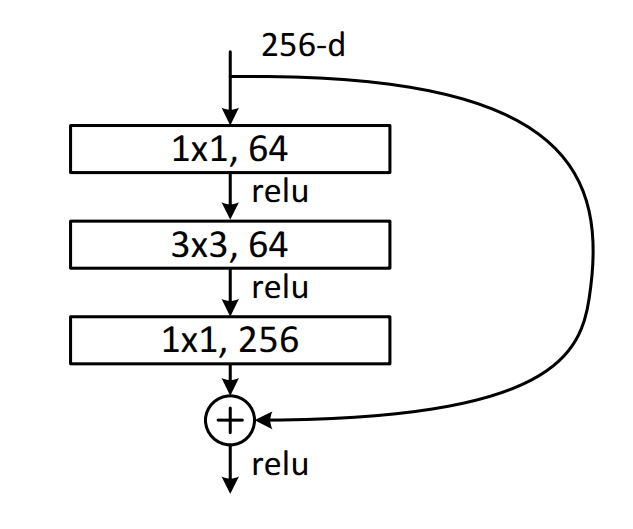
\includegraphics[width=0.3\textwidth]{figures/bottleneck}
\caption{
ResNet \cite{ResNet} \enquote{bottleneck} convolutional block introduced to reduce computational
complexity in deeper network variants, shown here with 256 input and output channels.
Figure from \cite{ResNet}.
}
\label{figure:bottleneck}
\end{figure}

\subsection{Region-based convolutional networks}
\label{ssec:rcnn}
We now give an overview of region-based convolutional networks, which are currently by far the
most popular deep networks for object detection, and have recently also been applied to instance segmentation.

\paragraph{R-CNN}
Region-based convolutional networks (R-CNNs) \cite{RCNN} use a non-learned algorithm external to a standard encoder CNN
for computing \emph{region proposals} in the shape of 2D bounding boxes, which represent regions that may contain an object.
For each of the region proposals, the input image is cropped using the regions bounding box and the crop is
passed through a CNN, which performs classification of the object (or non-object, if the region shows background).

\paragraph{Fast R-CNN}
The original R-CNN involves computing one forward pass of the CNN for each of the region proposals,
which is costly, as there is generally a large number of proposals.
Fast R-CNN \cite{FastRCNN} significantly reduces computation by performing only a single forward pass with the whole image
as input to the CNN (compared to the sequential input of crops in the case of R-CNN).
Then, fixed size (H $\times$ W) feature maps are extracted from the compressed feature map of the image,
each corresponding to one of the proposal bounding boxes.
The extracted per-RoI feature maps are collected into a batch and passed into a small Fast R-CNN
\emph{head} network, which performs classification and prediction of refined boxes for all regions in one forward pass.
The extraction technique is called \emph{RoI pooling}. In RoI pooling, the RoI bounding box window over the full image features
is divided into a H $\times$ W grid of cells. For each cell, the values of the underlying
full image feature map are max-pooled to yield the output value at this cell.
Thus, given region proposals, the per-region computation is reduced to a single pass through the complete network,
speeding up the system by two orders of magnitude at inference time and one order of magnitude
at training time.

\paragraph{Faster R-CNN}
After streamlining the CNN components, Fast R-CNN is limited by the speed of the region proposal
algorithm, which has to be run prior to the network passes and makes up a large portion of the total
processing time.
The Faster R-CNN object detection system \cite{FasterRCNN} unifies the generation of region proposals and subsequent box refinement and
classification into a single deep network, leading to faster processing when compared to Fast R-CNN
and again, improved accuracy.
This unified network operates in two stages.
In the \emph{first stage}, one forward pass is performed on the \emph{backbone} network,
which is a deep feature encoder CNN with the original image as input.
Next, the \emph{backbone} output features are passed into a small, fully convolutional \emph{Region Proposal Network (RPN)} head, which
predicts objectness scores and regresses bounding boxes at each of its output positions.
At any of the $h \times w$ output positions of the RPN head,
$N_a$ bounding boxes with their objectness scores are predicted as offsets relative to a fixed set of $N_a$ \emph{anchors} with different
aspect ratios and scales. Thus, there are $N_a \times h \times w$ reference anchors in total.
In Faster R-CNN, $N_a = 9$, with 3 scales corresponding
to anchor boxes of areas of $\{128^2, 256^2, 512^2\}$ pixels and 3 aspect ratios,
$\{1:2, 1:1, 2:1\}$. For the ResNet Faster R-CNN backbone, we generally have a stride of 16
with respect to the input image at the RPN output (Table \ref{table:maskrcnn_resnet}).

For each RPN prediction at a given position, the objectness score tells us how likely it is to correspond to a detection.
The region proposals can then be obtained as the N highest scoring RPN predictions.

Then, the \emph{second stage} corresponds to the original Fast R-CNN head network, performing classification
and bounding box refinement for each of the region proposals, which are now obtained
from the RPN instead of being pre-computed by some external algorithm.
As in Fast R-CNN, RoI pooling is used to extract one fixed size feature map for each of the region proposals.

\paragraph{Mask R-CNN}
Faster R-CNN and the earlier systems detect and classify objects at bounding box granularity.
However, it can be helpful to know class and object (instance) membership of all individual pixels,
which generally involves computing a binary mask for each object instance specifying which pixels belong
to that object. This problem is called \emph{instance segmentation}.
Mask R-CNN \cite{MaskRCNN} extends the Faster R-CNN system to instance segmentation by predicting
fixed resolution instance masks within the bounding boxes of each detected object.
This is done by simply extending the Faster R-CNN head with multiple convolutions, which
compute a pixel-precise binary mask for each instance.
The basic Mask R-CNN ResNet-50 architecture is shown in Table \ref{table:maskrcnn_resnet}.
Note that the per-class masks logits are put through a sigmoid layer, and thus there is no
comptetition between classes for the mask prediction branch.

One important technical aspect of Mask R-CNN is the replacement of RoI pooling with
bilinear sampling for extracting the RoI features, which is much more precise.
%In RoI pooling, at the borders, the bins for max-pooling are not aligned with the actual pixel
%boundary of the bounding box.


{
%\begin{table}[t]
%\centering
\begin{longtable}{llr}
\toprule
\textbf{Output} & \textbf{Layer Operations} & \textbf{Output Dimensions} \\
\midrule\midrule
& input image & H $\times$ W $\times$ C \\
\midrule
C$_4$ & ResNet-50 \{up to C$_4$\} (Table \ref{table:resnet})  & $\tfrac{1}{16}$ H $\times$ $\tfrac{1}{16}$ W $\times$ 1024 \\
\midrule
\multicolumn{3}{c}{\textbf{Region Proposal Network (RPN)}}\\
\midrule
R$_0$ & From C$_4$: 1 $\times$ 1 conv, 512 & $\tfrac{1}{16}$ H $\times$ $\tfrac{1}{16}$ W $\times$ 512 \\
& 1 $\times$ 1 conv, 4 & $\tfrac{1}{16}$ H $\times$ $\tfrac{1}{16}$ W $\times$ $N_a \cdot$ 4 \\
& flatten & A $\times$ 4 \\
boxes$_{\mathrm{RPN}}$ & decode bounding boxes (Eq. \ref{eq:pred_bounding_box}) & A $\times$ 4\\
& From R$_0$: 1 $\times$ 1 conv, 2 & $\tfrac{1}{16}$ H $\times$ $\tfrac{1}{16}$ W $\times$ $N_a \cdot$ 2 \\
& flatten & A $\times$ 2 \\
scores$_{\mathrm{RPN}}$& softmax & A $\times$ 2 \\
ROI$_{\mathrm{RPN}}$ & sample boxes$_{\mathrm{RPN}}$ and scores$_{\mathrm{RPN}}$ & N$_{RoI}$ $\times$ 6 \\
\midrule
\multicolumn{3}{c}{\textbf{RoI Head}}\\
\midrule
& From C$_4$ with ROI$_{\mathrm{RPN}}$: RoI extraction & N$_{RoI}$ $\times$ 7 $\times$ 7 $\times$ 1024 \\
R$_1$& ResNet-50 \{C$_5$ without stride\} (Table \ref{table:resnet})  & N$_{RoI}$ $\times$ 7 $\times$ 7 $\times$ 2048 \\
ave & average pool & N$_{RoI}$ $\times$ 2048 \\
& From ave: fully connected, N$_{cls}$ $\cdot$ 4 & N$_{RoI}$ $\times$ N$_{cls}$ $\cdot$ 4\\
boxes & decode bounding boxes (Eq. \ref{eq:pred_bounding_box}) & N$_{RoI}$ $\times$ N$_{cls}$ $\cdot$ 4\\
& From ave: fully connected, N$_{cls}$ & N$_{RoI}$ $\times$ N$_{cls}$ \\
classes& softmax, N$_{cls}$ & N$_{RoI}$ $\times$ N$_{cls}$ \\
\midrule
\multicolumn{3}{c}{\textbf{RoI Head: Masks}}\\
\midrule
& From R$_1$: 2 $\times$ 2 deconv, 256, stride 2 & N$_{RoI}$ $\times$ 14 $\times$ 14 $\times$ 256 \\
& 1 $\times$ 1 conv, N$_{cls}$ & N$_{RoI}$ $\times$ 14 $\times$ 14 $\times$ N$_{cls}$ \\
masks & sigmoid, N$_{cls}$ & N$_{RoI}$ $\times$ 28 $\times$ 28 $\times$ N$_{cls}$ \\

\bottomrule

\caption {
Mask R-CNN \cite{MaskRCNN} ResNet-50 \cite{ResNet} architecture.
Note that this is equivalent to the Faster R-CNN architecture if the mask
head is left out. In Mask R-CNN, bilinear sampling is used for RoI extraction,
whereas Faster R-CNN used RoI pooling.
}
\label{table:maskrcnn_resnet}
\end{longtable}
%\end{table}
}

\paragraph{Feature Pyramid Networks}
In Faster R-CNN, a single feature map is used as a source of all RoIs, independent
of the size of the bounding box of the RoI.
However, for small objects, the C$_4$ (see Table \ref{table:maskrcnn_resnet}) features
might have lost too much spatial information to properly predict the exact bounding
box and a high resolution mask. Likewise, for very big objects, the fixed size
RoI window might be too small to cover the region of the feature map containing
information for this object.
As a solution to this, the Feature Pyramid Network (FPN) \cite{FPN} enable features
of an appropriate scale to be used, depending of the size of the bounding box.
For this, a pyramid of feature maps is created on top of the ResNet \cite{ResNet}
encoder by combining bilinear upsampled feature maps coming from the bottleneck
with lateral skip connections from the encoder.
The Mask R-CNN ResNet-50-FPN variant is shown in Table \ref{table:maskrcnn_resnet_fpn}.
Instead of a single RPN head with anchors at 3 scales and 3 aspect ratios,
the FPN variant has one RPN head after each of the pyramid levels P$_2$ ... P$_6$.
At each output position of the resulting RPN pyramid, bounding boxes are predicted
with respect to 3 anchor aspect ratios $\{1:2, 1:1, 2:1\}$ and a single scale ($N_a = 3$).
For P$_2$, P$_3$, P$_4$, P$_5$, P$_6$,
the scale corresponds to anchor bounding boxes of areas $32^2, 64^2, 128^2, 256^2, 512^2$,
respectively.
Note that there is no need for multiple anchor scales per anchor position anymore,
as the RPN heads themselves correspond to multiple scales.
Now, in the RPN, higher resolution feature maps can be used for regressing smaller
bounding boxes. For example, boxes of area close to $32^2$ are predicted using P$_2$,
which has a stride of $4$ with respect to the input image.
Most importantly, the RoI features can now be extracted at the pyramid level $P_j$ appropriate for a
RoI bounding box with size $h \times w$,
\begin{equation}
j = \log_2(\sqrt{w \cdot h} / 224). %TODO complete
\label{eq:level_assignment}
\end{equation}


{
%\begin{table}[t]
%\centering
\begin{longtable}{llr}
\toprule
\textbf{Output} & \textbf{Layer Operations} & \textbf{Output Dimensions} \\
\midrule\midrule
& input image & H $\times$ W $\times$ C \\
\midrule
C$_5$ & ResNet-50 (Table \ref{table:resnet})  & $\tfrac{1}{32}$ H $\times$ $\tfrac{1}{32}$ W $\times$ 1024 \\
\midrule
\multicolumn{3}{c}{\textbf{Feature Pyramid Network (FPN)}}\\
\midrule
P$_5$ & From C$_5$: 1 $\times$ 1 conv, 256 & $\tfrac{1}{32}$ H $\times$ $\tfrac{1}{32}$ W $\times$ 256 \\
P$_4$ & $\begin{bmatrix}\textrm{skip from C$_4$}\end{bmatrix}_p$ & $\tfrac{1}{16}$ H $\times$ $\tfrac{1}{16}$ W $\times$ 256 \\
P$_3$ & $\begin{bmatrix}\textrm{skip from C$_3$}\end{bmatrix}_p$ & $\tfrac{1}{8}$ H $\times$ $\tfrac{1}{8}$ W $\times$ 256 \\
P$_2$ & $\begin{bmatrix}\textrm{skip from C$_2$}\end{bmatrix}_p$ & $\tfrac{1}{4}$ H $\times$ $\tfrac{1}{4}$ W $\times$ 256 \\
P$_6$ & From P$_5$: 2 $\times$ 2 subsample, 256 & $\tfrac{1}{64}$ H $\times$ $\tfrac{1}{64}$ W $\times$ 256 \\
\midrule
\multicolumn{3}{c}{\textbf{Region Proposal Network (RPN)}}\\
\midrule
\multicolumn{3}{c}{$\forall i \in \{2...6\}$}\\
& From P$_i$: 1 $\times$ 1 conv, 512 & $\tfrac{1}{2^i}$ H $\times$ $\tfrac{1}{2^i}$ W $\times$ 512 \\
& 1 $\times$ 1 conv, 6 & $\tfrac{1}{2^i}$ H $\times$ $\tfrac{1}{2^i}$ W $\times$ $N_a \cdot$ 6 \\
RPN$_i$& flatten & A$_i$ $\times$ 6 \\
\midrule
& From \{RPN$_2$ ... RPN$_6$\}: concatenate & A $\times$ 6 \\
& decode bounding boxes (Eq. \ref{eq:pred_bounding_box}) & A $\times$ 6 \\
ROI$_{\mathrm{RPN}}$ & sample bounding boxes \& scores & N$_{RoI}$ $\times$ 6 \\
\midrule
\multicolumn{3}{c}{\textbf{RoI Head}}\\
\midrule
R$_2$ & From \{P$_2$ ... P$_6$\} with ROI$_{\mathrm{RPN}}$: RoI extraction (Eq. \ref{eq:level_assignment}) & N$_{RoI}$ $\times$ 14 $\times$ 14 $\times$ 256 \\
& 2 $\times$ 2 max pool & N$_{RoI}$ $\times$ 7 $\times$ 7 $\times$ 256 \\
F$_1$ & $\begin{bmatrix}\textrm{fully connected}, 1024\end{bmatrix}$ $\times$ 2 & N$_{RoI}$ $\times$ 1024 \\
& From F$_1$: fully connected, N$_{cls}$ $\cdot$ 4 & N$_{RoI}$ $\times$ N$_{cls}$ $\cdot$ 4 \\
boxes & decode bounding boxes (Eq. \ref{eq:pred_bounding_box}) & N$_{RoI}$ $\times$ N$_{cls}$ $\cdot$ 4\\
& From F$_1$: fully connected, N$_{cls}$ & N$_{RoI}$ $\times$ N$_{cls}$ \\
classes& softmax, N$_{cls}$ & N$_{RoI}$ $\times$ N$_{cls}$ \\
\midrule
\multicolumn{3}{c}{\textbf{RoI Head: Masks}}\\
\midrule
& From R$_2$: $\begin{bmatrix}\textrm{3 $\times$ 3 conv} \end{bmatrix}$ $\times$ 4, 256 & N$_{RoI}$ $\times$ 14 $\times$ 14 $\times$ 256 \\
& 2 $\times$ 2 deconv, 256, stride 2 & N$_{RoI}$ $\times$ 28 $\times$ 28 $\times$ 256 \\
& 1 $\times$ 1 conv, N$_{cls}$ & N$_{RoI}$ $\times$ 28 $\times$ 28 $\times$ N$_{cls}$ \\
masks & sigmoid, N$_{cls}$ & N$_{RoI}$ $\times$ 28 $\times$ 28 $\times$ N$_{cls}$ \\
\bottomrule

\caption {
Mask R-CNN \cite{MaskRCNN} ResNet-50-FPN \cite{ResNet} architecture.
Operations enclosed in a []$_p$ block make up a single FPN
block (see Figure \ref{figure:fpn_block}).
}
\label{table:maskrcnn_resnet_fpn}
\end{longtable}
%\end{table}
}

\begin{figure}[t]
  \centering
  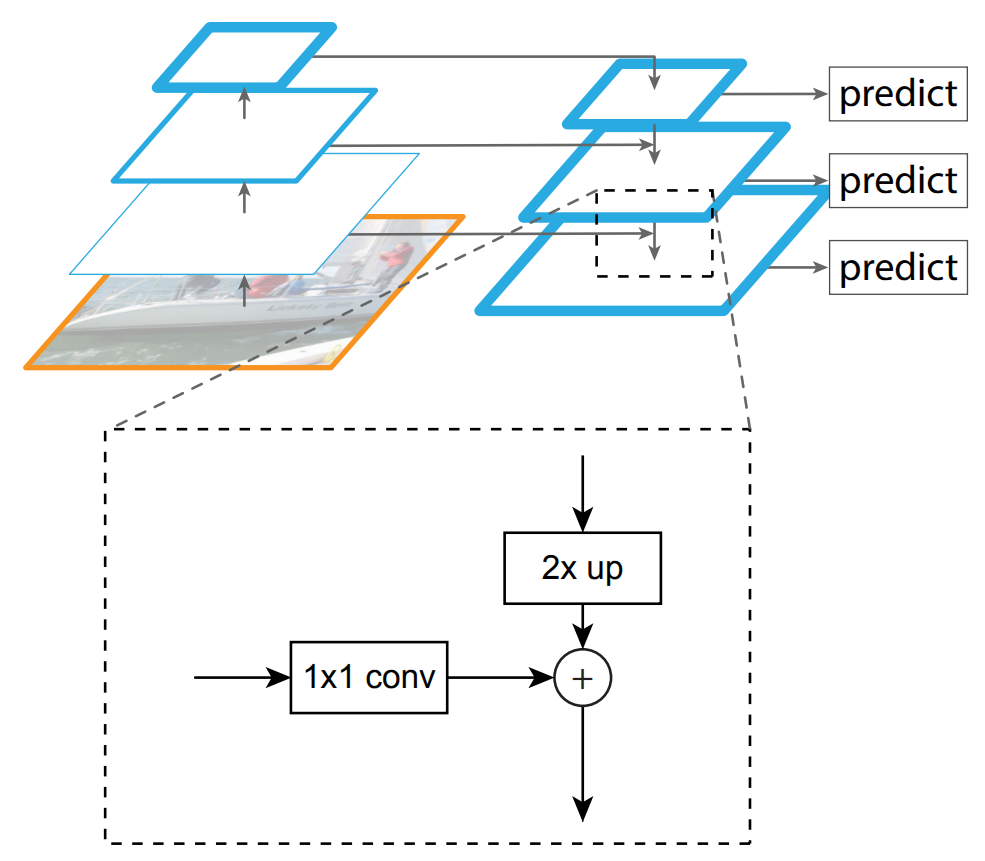
\includegraphics[width=0.3\textwidth]{figures/fpn}
\caption{
FPN block from \cite{FPN}.
Lower resolution features coming from the bottleneck are bilinearly upsampled
and added with higher resolution skip connections from the encoder.
Figure from \cite{FPN}.
}
\label{figure:fpn_block}
\end{figure}

\subsection{Training Mask R-CNN}
\paragraph{Loss definitions}
For regression, we define the smooth $\ell_1$ regression loss as
\begin{equation}
\ell_{reg}(x) =
\begin{cases}
0.5x^2 &\text{if |x| < 1} \\
|x| - 0.5 &\text{otherwise,}
\end{cases}
\end{equation}
which provides a certain robustness to outliers and will be used
frequently in the following chapters. For vector or tuple arguments, the sum of the componentwise scalar
losses is computed.
For classification we define $\ell_{cls}$ as the cross-entropy classification loss.

\label{ssec:rcnn_techn}
\paragraph{Bounding box regression}
All bounding boxes predicted by the RoI head or RPN are estimated as offsets
with respect to a reference bounding box. In the case of the RPN,
the reference bounding box is one of the anchors, and refined bounding boxes from the RoI head are
predicted relative to the RPN output bounding boxes.
Let $(x, y, w, h)$ be the top left coordinates, height and width of the bounding box
to be predicted. Likewise, let $(x^*, y^*, w^*, h^*)$ be the ground truth bounding
box and let $(x_r, y_r, w_r, h_r)$ be the reference bounding box.
The ground truth \emph{box encoding} $b_e^*$ is then defined as
\begin{equation}
b_e^* = (b_x^*, b_y^*, b_w^*, b_h^*),
\end{equation}
where
\begin{equation*}
b_x^* = \frac{x^* - x_r}{w_r},
\end{equation*}
\begin{equation*}
b_y^* = \frac{y^* - y_r}{h_r},
\end{equation*}
\begin{equation*}
b_w^* = \log \left( \frac{w^*}{w_r} \right),
\end{equation*}
\begin{equation*}
b_h^* = \log \left( \frac{h^*}{h_r} \right),
\end{equation*}
which represents the regression target for the bounding box
outputs of the network.

Thus, for each bounding box prediction, the network predicts the box encoding $b_e$,
\begin{equation}
b_e = (b_x, b_y, b_w, b_h),
\end{equation}
where
\begin{equation*}
b_x = \frac{x - x_r}{w_r},
\end{equation*}
\begin{equation*}
b_y = \frac{y - y_r}{h_r},
\end{equation*}
\begin{equation*}
b_w = \log \left( \frac{w}{w_r} \right),
\end{equation*}
\begin{equation*}
b_h = \log \left( \frac{h}{h_r} \right).
\end{equation*}

At test time, to get from a predicted box encoding $b_e$ to the predicted bounding box $b$,
the definitions above can be inverted,
\begin{equation}
b = (x, y, w, h),
\label{eq:pred_bounding_box}
\end{equation}
where
\begin{equation*}
x = b_x \cdot w_r + x_r,
\end{equation*}
\begin{equation*}
y = b_y \cdot b_r + y_r,
\end{equation*}
\begin{equation*}
w = \exp(b_w) \cdot w_r,
\end{equation*}
\begin{equation*}
h = \exp(b_h) \cdot h_r,
\end{equation*}
and thus the bounding box is obtained as the reference bounding box adjusted by
the predicted relative offsets and scales.

\paragraph{Supervision of the RPN}
A positive RPN proposal is defined as one with a IoU of at least $0.7$ with
a ground truth bounding box. For training the RPN, $N_{RPN} = 256$  positive and negative
examples are randomly sampled from the set of all RPN proposals,
with at most $50\%$ positive examples (if there are less positive examples,
more negative examples are used instead).
For examples selected in this way, a regression loss is computed between
predicted and ground truth bounding box encoding, and a classification loss
is computed for the predicted objectness.
Specifically, let $s_i^* = 1$ if proposal $i$ is positive and $s_i^* = 0$ if
it is negative, let $s_i$ be the predicted objectness score and $b_i$, $b_i^*$ the
predicted and ground truth bounding box encodings.
Then, the RPN loss is computed as
\begin{equation}
L_{RPN} = L_{obj} + L_{box}^{RPN},
\end{equation}
where
\begin{equation}
L_{obj} = \frac{1}{N_{RPN}} \sum_{i=1}^{N_{RPN}} \ell_{cls}(s_i, s_i^*),
\end{equation}
\begin{equation}
L_{box}^{RPN} = \frac{1}{N_{RPN}^{pos}} \sum_{i=1}^{N_{RPN}} s_i^* \cdot \ell_{reg}(b_i^* - b_i),
\end{equation}
and
\begin{equation}
N_{RPN}^{pos} = \sum_{i=1}^{N_{pos}} s_i^*
\end{equation}
is the number of positive examples. Note that the bounding box loss is only
active for positive examples, and that the classification loss is computed
between the classes $\{\textrm{object},\textrm{non-object}\}$.

\paragraph{Supervision of the Mask R-CNN RoI head}
For selecting RoIs to train the RoI head network, a foreground example
is defined as one with a IoU of at least $0.5$ with
a ground truth bounding box, and a background example is defined as
one with a maximum IoU in $[0.1, 0.5)$.
A total of 64 (without FPN) or 512 (with FPN) RoIs are sampled, with
at most $25\%$ foreground examples.
Now, let $c_i^*$ be the ground truth object class, where $c_i = 0$
for background examples and $c_i \in \{1, ..., N_{cls}\}$ for foreground examples,
and let $c_i$ be the class prediction.
Now, for any foreground RoI, let $b_i^*$ be the ground truth bounding box encoding and $b_i$
the predicted refined box encoding for class $c_i^*$.
Additionally, for any foreground RoI, let $m_i$ be the predicted $m \times m$ mask for class $c_i^*$
and $m_i^*$ the $m \times m$ mask target with values in $\{0,1\}$, where the mask target is cropped and resized from
the binary ground truth mask using the RPN proposal bounding box.
Then, the ROI loss is computed as
\begin{equation}
L_{RoI} = L_{cls} + L_{box} + L_{mask}
\end{equation}
where
\begin{equation}
L_{cls} = \frac{1}{N_{RoI}} \sum_{i=1}^{N_{RoI}} \ell_{cls}(c_i, c_i^*),
\end{equation}
is the average cross-entropy classification loss,
\begin{equation}
L_{box} = \frac{1}{N_{RoI}^{fg}} \sum_{i=1}^{N_{RoI}} [c_i^* \geq 1] \cdot \ell_{reg}(b_i^* - b_i)
\end{equation}
is the average smooth-$\ell_1$ bounding box regression loss,
\begin{equation}
L_{mask} = \frac{1}{N_{RoI}^{fg}} \sum_{i=1}^{N_{RoI}} [c_i^* \geq 1] \cdot \ell_{cls}(m_i,m_i^*)
\end{equation}
is the average binary cross-entropy mask loss,
\begin{equation}
N_{RoI}^{fg} = \sum_{i=1}^{N_{RoI}} [c_i^* \geq 1]
\end{equation}
is the number of foreground examples, and
\begin{equation}
[c_i^* \geq 1] =
\begin{cases}
1 &\text{$c_i^* \geq 1$} \\
0 &\text{otherwise}
\end{cases}
\end{equation}
is the Iverson bracket indicator function. Thus, the bounding box and mask
losses are only enabled for the foreground RoIs. Note that the bounding box and mask predictions
for all classes other than $c_i^*$ are not penalized.

\paragraph{Inference}
During inference, the 300 (without FPN) or 1000 (with FPN) highest scoring region proposals
from the RPN are selected. The corresponding features are extracted from the backbone, as during training, by using the RPN bounding boxes,
and passed through the RoI bounding box refinement and classification heads
(but not through the mask head).
After this, non-maximum supression (NMS) is applied to predicted RoIs with predicted non-background class,
with a maximum IoU of 0.7.
Then, the mask head is applied to the 100 highest scoring (after NMS) refined boxes,
after again extracting the corresponding features.
Thus, during inference, the features for the mask head are extracted using the refined
bounding boxes, instead of the RPN bounding boxes. This is important for not
introducing any misalignment, as we want to create the instance mask inside of the
more precise, refined detection bounding boxes.


\section{Motion R-CNN}
\parindent 2em
\onehalfspacing

\label{sec:approach}

\subsection{Motion R-CNN}
\label{ssec:model}

Building on Mask R-CNN \cite{MaskRCNN},
we estimate per-object motion by predicting the 3D motion of each detected object.
For this, we extend Mask R-CNN in two straightforward ways.
First, we modify the backbone network and provide two frames to the R-CNN system
in order to enable image matching between the consecutive frames.
Second, we extend the Mask R-CNN RoI head to predict a 3D motion for each
region proposal. Tables \ref{table:motionrcnn_resnet} and \ref{table:motionrcnn_resnet_fpn}
show our Motion R-CNN networks based on Mask R-CNN ResNet and Mask R-CNN ResNet-FPN,
respectively.

{\begin{table}[h]
\centering
\begin{tabular}{llr}
\toprule
\textbf{Output} & \textbf{Layer Operations} & \textbf{Output Dimensions} \\
\midrule\midrule
& input images & H $\times$ W $\times$ C \\
\midrule
C$_4$ & ResNet \{up to C$_4$\} (Table \ref{table:resnet}) & $\tfrac{1}{16}$ H $\times$ $\tfrac{1}{16}$ W $\times$ 1024 \\
\midrule
\multicolumn{3}{c}{\textbf{Region Proposal Network (RPN)} (Table \ref{table:maskrcnn_resnet})}\\
\midrule
\multicolumn{3}{c}{\textbf{Camera Motion Network}}\\
\midrule
& From C$_4$: ResNet \{C$_6$\} (Table \ref{table:resnet}) & $\tfrac{1}{64}$ H $\times$ $\tfrac{1}{64}$ W $\times$ 2048 \\
& bilinear resize, 7 $\times$ 7 & 7 $\times$ 7 $\times$ 512 \\
& flatten & 1 $\times$ 7 $\cdot$ 7 $\cdot$ 512 \\
T$_0$ & $\begin{bmatrix}\textrm{fully connected}, 1024\end{bmatrix}$ $\times$ 2  & 1 $\times$ 1024 \\

$R_t^{cam}$& From T$_0$: fully connected, 3 & 1 $\times$ 3 \\
$t_t^{cam}$& From T$_0$: fully connected, 3 & 1 $\times$ 3 \\
& From T$_0$: fully connected, 2 & 1 $\times$ 2 \\
$o_t^{cam}$& softmax, 2 & 1 $\times$ 2 \\
\midrule
\multicolumn{3}{c}{\textbf{RoI Head \& RoI Head: Masks} (Table \ref{table:maskrcnn_resnet})}\\
\midrule
\multicolumn{3}{c}{\textbf{RoI Head: Motions}}\\
\midrule
%& From M$_0$: flatten & N$_{RoI}$ $\times$ 7 $\cdot$ 7 $\cdot$ 256 \\
T$_1$ & From ave: $\begin{bmatrix}\textrm{fully connected}, 1024\end{bmatrix}$ $\times$ 2 & N$_{RoI}$ $\times$ 1024 \\
$\forall k: R_t^k$ & From T$_1$: fully connected, 3 & N$_{RoI}$ $\times$ 3 \\
$\forall k: t_t^k$ & From T$_1$: fully connected, 3 & N$_{RoI}$ $\times$ 3 \\
$\forall k: p_t^k$ & From T$_1$: fully connected, 3 & N$_{RoI}$ $\times$ 3 \\
& From T$_1$: fully connected, 2 & N$_{RoI}$ $\times$ 2 \\
$\forall k: o_t^k$ & softmax, 2 & N$_{RoI}$ $\times$ 2 \\

\bottomrule
\end{tabular}

\caption {
Motion R-CNN ResNet architecture based on the Mask R-CNN
ResNet architecture (Table \ref{table:maskrcnn_resnet}).
We use ReLU activations after all hidden layers and
additonally dropout with $p = 0.5$ after all fully-connected hidden layers.
}
\label{table:motionrcnn_resnet}
\end{table}
}

{
\begin{table}[h]
\centering
\begin{tabular}{llr}
\toprule
\textbf{Output} & \textbf{Layer Operations} & \textbf{Output Dimensions} \\
\midrule\midrule
& input images & H $\times$ W $\times$ C \\
\midrule
C$_6$ & ResNet (Table \ref{table:resnet}) & $\tfrac{1}{64}$ H $\times$ $\tfrac{1}{64}$ W $\times$ 2048 \\
\midrule
\multicolumn{3}{c}{\textbf{RPN \& FPN} (Table \ref{table:maskrcnn_resnet_fpn})} \\
\midrule
\multicolumn{3}{c}{\textbf{Camera Motion Network}}\\
\midrule
& From C$_6$: 1 $\times$ 1 conv, 512 & $\tfrac{1}{32}$ H $\times$ $\tfrac{1}{32}$ W $\times$ 512 \\
& bilinear resize, 7 $\times$ 7 & 7 $\times$ 7 $\times$ 512 \\
& flatten & 1 $\times$ 7 $\cdot$ 7 $\cdot$ 512 \\
T$_2$ & $\begin{bmatrix}\textrm{fully connected}, 1024\end{bmatrix}$ $\times$ 2  & 1 $\times$ 1024 \\
$R_t^{cam}$& From T$_2$: fully connected, 3 & 1 $\times$ 3 \\
$t_t^{cam}$& From T$_2$: fully connected, 3 & 1 $\times$ 3 \\
& From T$_2$: fully connected, 2 & 1 $\times$ 2 \\
$o_t^{cam}$& softmax, 2 & 1 $\times$ 2 \\
\midrule
\multicolumn{3}{c}{\textbf{RoI Head \& RoI Head: Masks} (Table \ref{table:maskrcnn_resnet_fpn})} \\
\midrule
\multicolumn{3}{c}{\textbf{RoI Head: Motions}}\\
\midrule
%& From M$_1$: flatten & N$_{RoI}$ $\times$ 14 $\cdot$ 14 $\cdot$ 256 \\
T$_3$ & From F$_1$: $\begin{bmatrix}\textrm{fully connected}, 1024\end{bmatrix}$ $\times$ 2 & N$_{RoI}$ $\times$ 1024 \\
$\forall k: R_t^k$ & From T$_3$: fully connected, 3 & N$_{RoI}$ $\times$ 3 \\
$\forall k: t_t^k$ & From T$_3$: fully connected, 3 & N$_{RoI}$ $\times$ 3 \\
$\forall k: p_t^k$ & From T$_3$: fully connected, 3 & N$_{RoI}$ $\times$ 3 \\
& From T$_2$: fully connected, 2 & N$_{RoI}$ $\times$ 2 \\
$\forall k: o_t^k$ & softmax, 2 & N$_{RoI}$ $\times$ 2 \\

\bottomrule
\end{tabular}

\caption {
Motion R-CNN ResNet-FPN architecture based on the Mask R-CNN
ResNet-FPN architecture (Table \ref{table:maskrcnn_resnet_fpn}).
To obtain a larger bottleneck stride, we compute the feature pyramid starting
with C$_6$ instead of C$_5$ (thus, the subsampling from P$_5$ to P$_6$) is omitted.
The modifications are analogous to our Motion R-CNN ResNet,
but we still show the architecture for completeness.
Again, we use ReLU activations after all hidden layers and
additonally dropout with $p = 0.5$ after all fully-connected hidden layers.
}
\label{table:motionrcnn_resnet_fpn}
\end{table}
}

\paragraph{Motion R-CNN backbone}
Like Faster R-CNN and Mask R-CNN, we use a ResNet \cite{ResNet} variant as backbone network to compute feature maps from input imagery.

Inspired by FlowNetS \cite{FlowNet}, we make one modification to the ResNet backbone to enable image matching,
laying the foundation for our motion estimation. Instead of taking a single image as input to the backbone,
we depth-concatenate two temporally consecutive frames $I_t$ and $I_{t+1}$, yielding a input image map with six channels.
Alternatively, we also experiment with concatenating the camera space XYZ coordinates for each frame,
XYZ$_t$ and XYZ$_{t+1}$, into the input as well.
We do not introduce a separate network for computing region proposals and use our modified backbone network
as both first stage RPN and second stage feature extractor for extracting the RoI features.
Technically, our feature encoder network will have to learn a motion representation similar to
that learned by the FlowNet encoder, but the output will be computed in the
object-centric framework of a region based convolutional network head with a 3D parametrization.
Thus, in contrast to the dense FlowNet decoder, the estimated dense motion information
from the encoder is integrated for specific objects via RoI cropping and
processed by the RoI head for each object.

\paragraph{Per-RoI motion prediction}
We use a rigid 3D motion parametrization similar to the one used in SfM-Net and SE3-Nets \cite{SfmNet,SE3Nets}.
For the $k$-th object proposal, we predict the rigid transformation $\{R_t^k, t_t^k\}\in \mathbf{SE}(3)$
\footnote{$\mathbf{SE}(3)$ refers to the Special Euclidean Group representing 3D rotations
and translations: $\{R, t|R \in \mathbf{SO}(3), t \in \mathbb{R}^3\}$}
of the object between the two frames $I_t$ and $I_{t+1}$, as well as the object pivot $p_t^k \in \mathbb{R}^3$ at time $t$.
We parametrize ${R_t^k}$ using an Euler angle representation,

\begin{equation}
R_t^k = R_t^{k,z}(\gamma) \cdot R_t^{k,x}(\alpha) \cdot R_t^{k,y}(\beta),
\end{equation}

where
\begin{equation}
R_t^{k,x}(\alpha) =
\begin{pmatrix}
  1 & 0 & 0 \\
  0 & \cos(\alpha) & -\sin(\alpha) \\
  0 & \sin(\alpha) & \cos(\alpha)
\end{pmatrix},
\end{equation}

\begin{equation}
R_t^{k,y}(\beta) =
\begin{pmatrix}
  \cos(\beta) & 0 & \sin(\beta) \\
  0 & 1 & 0 \\
  -\sin(\beta) & 0 & \cos(\beta)
\end{pmatrix},
\end{equation}

\begin{equation}
R_t^{k,z}(\gamma) =
\begin{pmatrix}
  \cos(\gamma) & -\sin(\gamma) & 0 \\
  \sin(\gamma) & \cos(\gamma) & 0 \\
  0 & 0 & 1
\end{pmatrix},
\end{equation}

and $\alpha, \beta, \gamma$ are the rotation angles in radians about the $x,y,z$-axis, respectively.

We then extend the Mask R-CNN head by adding a small fully-connected network for motion
prediction in addition to the fully-connected layers for
refined boxes and classes and the convolutional network for the masks.
Like for refined boxes and masks, we make one separate motion prediction for each class.
Each instance motion is predicted as a set of nine scalar parameters,
$\sin(\alpha)$, $\sin(\beta)$, $\sin(\gamma)$, $t_t^k$ and $p_t^k$,
where $\sin(\alpha)$, $\sin(\beta)$ and $\sin(\gamma)$ are clipped to $[-1, 1]$.
Here, we assume that motions between frames are relatively small
and that objects rotate at most 90 degrees in either direction along any axis,
which is in general a safe assumption for image sequences from videos.
All predictions are made in camera space, and translation and pivot predictions are in meters.
We additionally predict softmax scores $o_t^k$ for classifying the objects into
still and moving objects. As a postprocessing, for any object instance $k$ with predicted moving flag $o_t^k = 0$,
we set $\sin(\alpha) = \sin(\beta) = \sin(\gamma) = 0$ and $t_t^k = (0,0,0)^T$,
and thus predict an identity motion.


\paragraph{Camera motion prediction}
In addition to the object transformations, we optionally predict the camera motion $\{R_t^{cam}, t_t^{cam}\}\in \mathbf{SE}(3)$
between the two frames $I_t$ and $I_{t+1}$.
For this, we branch off a small fully-connected network from the bottleneck output of the backbone.
We again represent $R_t^{cam}$ using a Euler angle representation and
predict $\sin(\alpha)$, $\sin(\beta)$, $\sin(\gamma)$ and $t_t^{cam}$ in the same way as for the individual objects.
Again, we predict a softmax score $o_t^{cam}$ for differentiating between
a still and moving camera.

\subsection{Network design}

\label{ssec:design}
\paragraph{Camera motion network}
In our ResNet variant without FPN (Table \ref{table:motionrcnn_resnet}), the underlying
ResNet backbone is only computed up to the $C_4$ block, as otherwise the
feature resolution prior to RoI extraction would be reduced too much.
In our ResNet variant, we therefore first pass the $C_4$ features through a $C_5$
block to make the camera network of both variants comparable.
Then, in both, the ResNet and ResNet-FPN variant (Table \ref{table:motionrcnn_resnet_fpn}), we apply a additional
convolution to the $C_5$ features to reduce the number of inputs to the following
fully-connected layers.
Instead of averaging, we use bilinear resizing to bring the convolutional features
to a fixed size without losing all spatial information,
flatten them, and finally apply multiple fully-connected layers to compute the
camera motion prediction.

\paragraph{RoI motion head network}
In both of our network variants
(Tables \ref{table:motionrcnn_resnet} and \ref{table:motionrcnn_resnet_fpn}),
we compute the fully-connected network for motion prediction from the
flattened RoI features, which are also the basis for classification and
bounding box refinement.

\subsection{Supervision}
\label{ssec:supervision}

\paragraph{Per-RoI instance motion supervision with 3D instance motion ground truth}
The most straightforward way to supervise the object motions is by using ground truth
motions computed from ground truth object poses, which is in general
only practical when training on synthetic datasets.
Given the $k$-th foreground RoI, let $i_k$ be the index of the matched ground truth example with class $c_k^*$,
let $R^{k,c_k}, t^{k,c_k}, p^{k,c_k}, o^{k,c_k}$ be the predicted motion for class $c_k^*$
and $R^{gt,i_k}, t^{gt,i_k}, p^{gt,i_k}, o^{gt,i_k}$ the ground truth motion for the example $i_k$.
Note that we dropped the subscript $t$ to increase readability.
Similar to the camera pose regression loss in \cite{PoseNet2},
we use a variant of the $\ell_1$-loss to penalize the differences between ground truth and predicted
rotation, translation (and pivot, in our case). We found that the smooth $\ell_1$-loss
performs better in our case than the standard $\ell_1$-loss.
We then compute the RoI motion loss as

\begin{equation}
L_{motion} = \frac{1}{N_{RoI}^{fg}} \sum_k^{N_{RoI}} l_{p}^k + (l_{R}^k + l_{t}^k) \cdot o^{gt,i_k} + l_o^k,
\end{equation}
where
\begin{equation}
l_{R}^k = \ell_{reg} (R^{gt,i_k} - R^{k,c_k}),
\end{equation}
\begin{equation}
l_{t}^k = \ell_{reg} (t^{gt,i_k} - t^{k,c_k}),
\end{equation}
\begin{equation}
l_{p}^k = \ell_{reg} (p^{gt,i_k} - p^{k,c_k}).
\end{equation}
are the smooth $\ell_1$-loss terms for the predicted rotation, translation and pivot,
respectively and
\begin{equation}
l_o^k = \ell_{cls}(o_t^k, o^{gt,i_k}).
\end{equation}
is the cross-entropy loss for the predicted classification into moving and non-moving objects.

Note that we do not penalize the rotation and translation for objects with
$o^{gt,i_k} = 0$, which do not move between $t$ and $t+1$. We found that the network
may not reliably predict exact identity motions for still objects, which is
numerically more difficult to optimize than performing classification between
moving and non-moving objects and discarding the regression for the non-moving
ones. Also, analogous to masks and bounding boxes, the estimates for classes
other than $c_k^*$ are not penalized.

Now, our modified RoI loss is
\begin{equation}
L_{RoI} = L_{cls} + L_{box} + L_{mask} + L_{motion}.
\end{equation}

\paragraph{Camera motion supervision}
We supervise the camera motion with ground truth analogously to the
object motions, with the only difference being that we only have
a rotation and translation, but no pivot term for the camera motion.
If the ground truth shows that the camera is not moving, we again do not
penalize rotation and translation. For the camera, the loss is reduced to the
classification term in this case.

\paragraph{Per-RoI instance motion supervision \emph{without} 3D instance motion ground truth}
\begin{figure}[t]
  \centering
  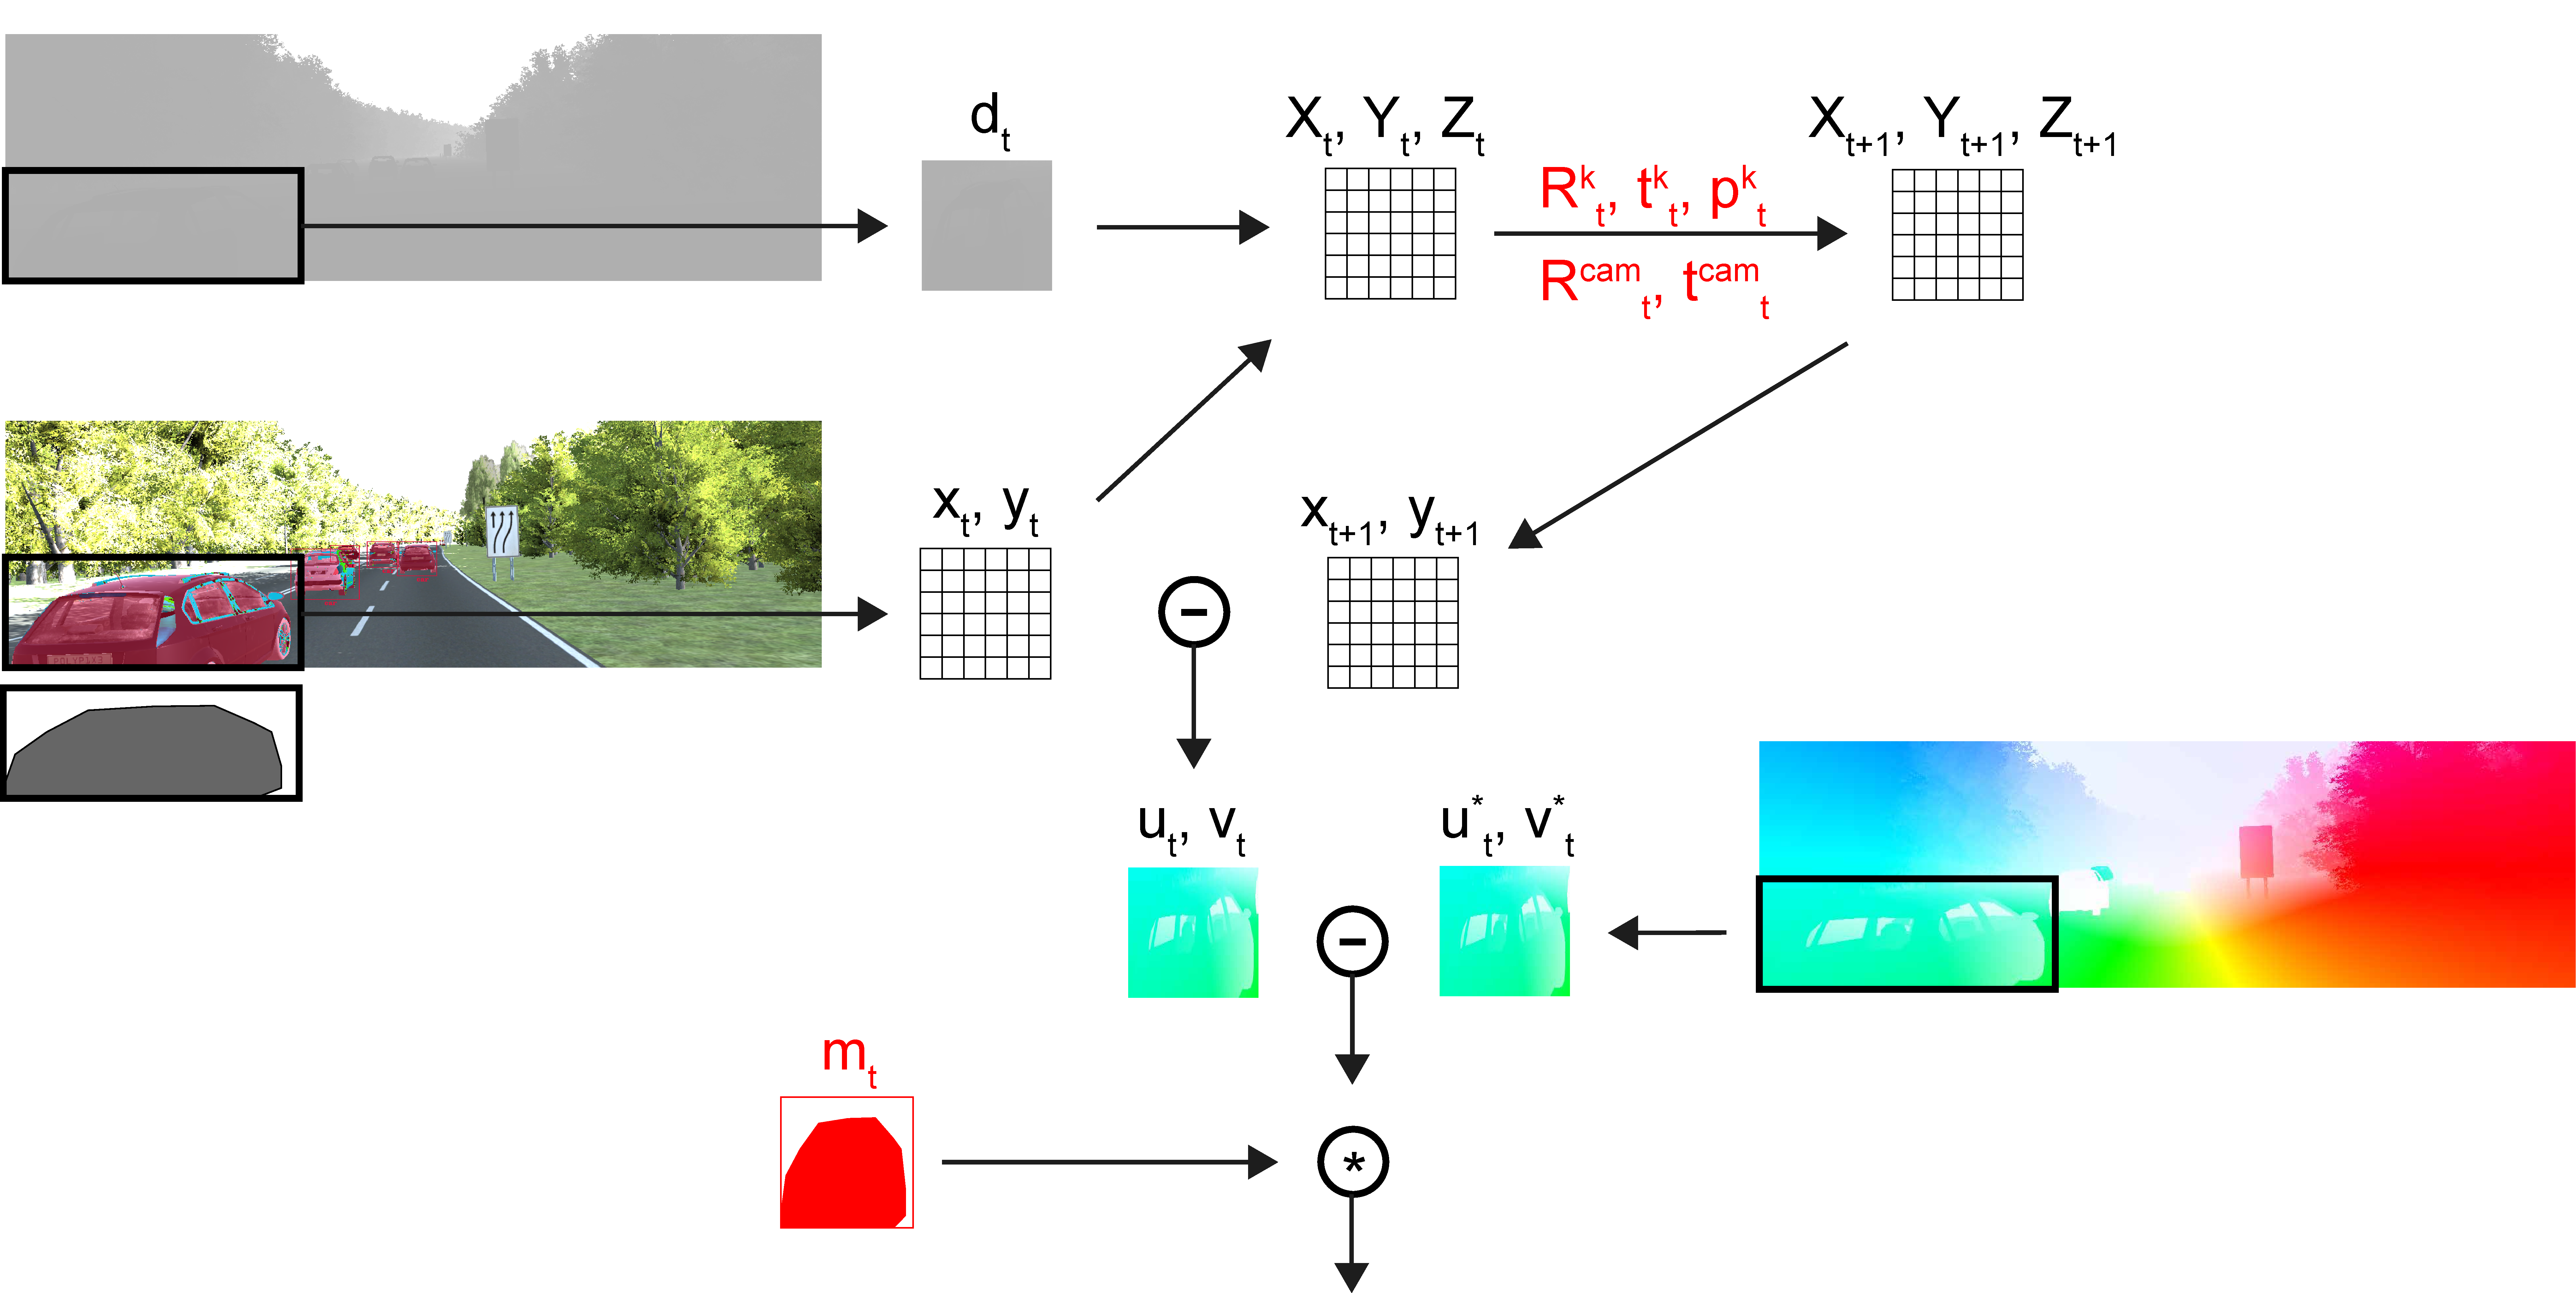
\includegraphics[width=\textwidth]{figures/flow_loss}
\caption{
Overview of the alternative, optical flow based loss for instance motion
supervision without 3D instance motion ground truth.
In contrast to SfM-Net, where a single optical flow field is
composed and penalized to supervise the motion prediction, our loss considers
the motion of all objects in isolation and composes a batch of flow windows
for the RoIs. Network predictions are shown in red.
}
\label{figure:flow_loss}
\end{figure}

A more general way to supervise the object motions is a re-projection
loss similar to the unsupervised loss in SfM-Net \cite{SfmNet},
which we can apply to coordinates within the object bounding boxes,
and which does not require ground truth 3D object motions.

In this case, for any RoI,
we generate a uniform $m \times m$ 2D grid of points inside the RPN proposal bounding box
with the same resolution as the predicted mask.
We use the same bounding box
to crop the corresponding region from the dense, full image depth map
and bilinearly resize the depth crop to the same resolution as the mask and point
grid.
We then compute the optical flow at each of the grid points by creating
a 3D point cloud from the point grid and depth crop. To this point cloud, we
apply the RoI's predicted motion, masked by the predicted mask.
Then, we apply the camera motion to the points, project them back to 2D
and finally compute the optical flow at each point as the difference of the initial and re-projected 2D grids.
Note that we batch this computation over all RoIs, so that we only perform
it once per forward pass. Figure \ref{figure:flow_loss} illustrates the approach.
The mathematical details for the 3D transformations and mappings between 2D and 3D are analogous to the
dense, full image flow composition in the following subsection, so we will not
include them here. The only differences are that there is no sum over objects during
the point transformation based on instance motion, as we consider the single object
corresponding to an RoI in isolation, and that the masks are not resized to the
full image resolution, as
the depth crops and 2D point grid are at the same resolution as the predicted
$m \times m$ mask.

For each RoI, we can now compute $L_{RoI}$ and thus supervise the object motion
by penalizing the $m \times m$ optical flow grid.
If there is optical flow ground truth available, we can use the RoI bounding box to
crop and resize a region from the ground truth optical flow to match the RoI's
optical flow grid and penalize the difference between the flow grids with an $\ell_1$-loss.

However, we can also use the re-projection loss without optical flow ground truth
to train the motion prediction in an unsupervised manner, similar to \cite{SfmNet}.
In this case, we use the bounding box to crop and resize a corresponding region
from the first image $I_t$ and bilinearly sample a region from the second image $I_{t+1}$
using the 2D grid displaced with the predicted flow grid. Then, we can penalize the difference
between the resulting image crops, for example, with a census loss \cite{CensusTerm,UnFlow}.
For more details on differentiable bilinear sampling for deep learning, we refer the reader to
\cite{STN}.

When compared to supervision with motion ground truth, a re-projection
loss could benefit motion regression by removing any loss balancing issues between the
rotation, translation and pivot terms \cite{PoseNet2},
which can make it interesting even when 3D motion ground truth is available.

\subsection{Training and inference}
\label{ssec:training_inference}
\paragraph{Training}
We train the Motion R-CNN RPN and RoI heads in the exact same way as described for Mask R-CNN.
We additionally compute the camera and instance motion losses and concatenate additional
information into the network input, but otherwise do not modify the training procedure
and sample proposals and RoIs in the exact same way.

\paragraph{Inference}
During inference, we proceed analogously to Mask R-CNN.
In the same way as the RoI mask head, at test time, we compute the RoI motion head
from the features extracted with refined bounding boxes.
Additionally, we use the \emph{predicted} binarized masks for each RoI to mask the
extracted RoI features before passing them into the motion head.
The intuition behind that is that we want to mask out (set to zero) any positions in the
extracted feature window which belong to the background. Then, the RoI motion
head aggregates the motion (image matching) information from the backbone
over positions localized within the object only, but not over positions belonging
to the background, which should not influence the final object motion estimate.

Again, as for masks and bounding boxes in Mask R-CNN,
the predicted output object motions are the predicted object motions for the
highest scoring class.

\subsection{Dense flow from motion}
\label{ssec:postprocessing}
As a postprocessing, we compose a dense optical flow map from the outputs of our Motion R-CNN network.
Given the depth map $d_t$ for frame $I_t$, we first create a 3D point cloud in camera space at time $t$,
where
\begin{equation}
P_t =
\begin{pmatrix}
X_t \\ Y_t \\ Z_t
\end{pmatrix}
=
\frac{d_t}{f}
\begin{pmatrix}
x_t - c_0 \\ y_t - c_1 \\ f
\end{pmatrix},
\end{equation}
is the 3D coordinate at $t$ corresponding to the point with pixel coordinates $x_t, y_t$,
which range over all coordinates in $I_t$.
For now, the depth map is always assumed to come from ground truth.

Given $k$ detections with predicted motions as above, we transform all points within the bounding
box of a detected object according to the predicted motion of the object.

We first define the \emph{full image} mask $M_t^k$ for object k,
which can be computed from the predicted box mask $m_t^k$ by bilinearly resizing
$m_t^k$ to the width and height of the predicted bounding box and then copying the values
of the resized mask into a full resolution mask initialized with zeros,
starting at the top-left coordinate of the predicted bounding box.
Then, given the predicted motions $(R_t^k, t_t^k)$ as well as $p_t^k$ for all objects,
\begin{equation}
P'_{t+1} =
P_t + \sum_1^{k} M_t^k\left\{ R_t^k \cdot (P_t - p_t^k) + p_t^k + t_t^k - P_t \right\}
\end{equation}
These motion predictions are understood to have already taken into account
the classification into moving and still objects,
and we thus, as described above, have identity motions for all objects with $o_t^k = 0$.

Next, we transform all points given the camera transformation $\{R_t^c, t_t^c\} \in \mathbf{SE}(3)$,

\begin{equation}
\begin{pmatrix}
X_{t+1} \\ Y_{t+1} \\ Z_{t+1}
\end{pmatrix}
= P_{t+1} = R_t^c \cdot P'_{t+1} + t_t^c
\end{equation}.

Note that in our experiments, we either use the ground truth camera motion to focus
on evaluating the object motion predictions or the predicted camera motion to evaluate
the complete motion estimates. We will always state which variant we use in the experimental section.

Finally, we project the transformed 3D points at time $t+1$ to pixel coordinates again,
\begin{equation}
\begin{pmatrix}
x_{t+1} \\ y_{t+1}
\end{pmatrix}
=
\frac{f}{Z_{t+1}}
\begin{pmatrix}
X_{t+1} \\ Y_{t+1}
\end{pmatrix}
+
\begin{pmatrix}
c_0 \\ c_1
\end{pmatrix}.
\end{equation}
We can now obtain the optical flow between $I_t$ and $I_{t+1}$ at each point as
\begin{equation}
\begin{pmatrix}
u \\ v
\end{pmatrix}
=
\begin{pmatrix}
x_{t+1} - x_{t} \\ y_{t+1} - y_{t}
\end{pmatrix}.
\end{equation}


\section{Experiments}
\parindent 2em
\onehalfspacing

\subsection{Implementation}
Our networks and loss functions are implemented using built-in TensorFlow
functions \cite{TensorFlow}, enabling us to use automatic differentiation for all gradient
computations. To make our code easy to extend and flexible, we build on
the TensorFlow Object detection API \cite{TensorFlowObjectDetection}, which provides a Faster R-CNN baseline
implementation.
On top of this, we implemented Mask R-CNN and the Feature Pyramid Network (FPN)
as well as the Motion R-CNN extensions for motion estimation and related evaluations
and postprocessings. In addition, we generated all ground truth for
Motion R-CNN in the form of TFRecords from the raw Virtual KITTI
data to enable fast loading during training.
Note that for RoI extraction and bilinear crop and resize operations,
we use the \texttt{tf.crop\_and\_resize} TensorFlow function with
interpolation set to bilinear.

\subsection{Datasets}
\label{ssec:datasets}

\paragraph{Virtual KITTI}
The synthetic Virtual KITTI dataset \cite{VKITTI} is a re-creation of the KITTI
driving scenario \cite{KITTI2012, KITTI2015}, rendered from virtual 3D street
scenes.
The dataset is made up of a total of 2126 frames from five different monocular
sequences recorded from a camera mounted on a virtual car.
Each sequence is rendered with varying lighting and weather conditions and
from different viewing angles, resulting in a total of 10 variants per sequence.
In addition to the RGB frames, a variety of ground truth is supplied.
For each frame, we are given a dense depth and optical flow map and the camera
extrinsics matrix. There are two annotated object classes, cars, and vans (N$_{cls}$ = 2).
For all cars and vans in the each frame, we are given 2D and 3D object bounding
boxes, instance masks, 3D poses, and various other labels.

This makes the Virtual KITTI dataset ideally suited for developing our joint
instance segmentation and motion estimation system, as it allows us to test
different components in isolation and progress to more and more complete
predictions up to supervising the full system on a single dataset.

For our experiments, we use the \emph{clone} sequences, which are rendered in a
way that most closely resembles the original KITTI dataset. We sample 100 examples
to be used as validation set. From the remaining 2026 examples,
we remove a small number of examples without object instances and use the resulting
data as training set.

\paragraph{Motion ground truth from 3D poses and camera extrinsics}
We will now describe how we use the ground truth poses and camera matrices from Virtual KITTI to
compute instance and camera motion ground truth.
For two consecutive frames $I_t$ and $I_{t+1}$,
let $[R_t^{ex}|t_t^{ex}]$
and $[R_{t+1}^{ex}|t_{t+1}^{ex}]$
be the camera extrinsics at the two frames.
We compute the ground truth camera motion
$\{R_{cam}^*, t_{cam}^*\} \in \mathbf{SE}(3)$ as

\begin{equation}
R_{cam}^* = R_{t+1}^{ex}  \cdot \mathrm{inv}(R_t^{ex}),
\end{equation}
\begin{equation}
t_{cam}^* = t_{t+1}^{ex}  - R_{cam}^* \cdot t_t^{ex}.
\end{equation}

Additionally, we define $o_{cam}^* \in \{ 0, 1 \}$,
\begin{equation}
o_{cam}^* =
\begin{cases}
1 &\text{if the camera pose changes between $t$ and $t+1$} \\
0 &\text{otherwise,}
\end{cases}
\end{equation}
which specifies the camera is moving in between the frames.

For any object $i$ visible in both frames, let
$(R_t^i, t_t^i)$ and $(R_{t+1}^i, t_{t+1}^i)$
be its orientation and position in camera space
at $I_t$ and $I_{t+1}$.
Note that the pose at $t$ is given with respect to the camera at $t$ and
the pose at $t+1$ is given with respect to the camera at $t+1$.

We define the ground truth pivot $p_k^* \in \mathbb{R}^3$ as

\begin{equation}
p_k^* = t_t^i
\end{equation}

and compute the ground truth object motion
$\{R_k^*, t_k^*\} \in \mathbf{SE}(3)$ as

\begin{equation}
R_k^* = \mathrm{inv}(R_{cam}^*) \cdot R_{t+1}^i \cdot \mathrm{inv}(R_t^i),
\end{equation}
\begin{equation}
t_k^* = t_{t+1}^{i}  - R_k^* \cdot t_t.
\end{equation}

As for the camera, we define $o_k^* \in \{ 0, 1 \}$,
\begin{equation}
o_k^* =
\begin{cases}
1 &\text{if the position of object i changes between $t$ and $t+1$} \\
0 &\text{otherwise,}
\end{cases}
\end{equation}
which specifies whether an object is moving in between the frames.

\paragraph{Evaluation metrics with motion ground truth}
To evaluate the 3D instance and camera motions on the Virtual KITTI validation
set, we introduce a few error metrics.
Given a foreground detection $k$ with an IoU of at least $0.5$ with a ground truth example,
let $R_k, t_k, p_k, o_k$ be the predicted motion for the predicted class $c_k$
and $R_k^*, t_k^*, p_k^*, o_k^*$ the motion ground truth for the best matching example.
Then, assuming there are $N$ such detections,
\begin{equation}
E_{R} = \frac{1}{N}\sum_k \arccos\left( \min\left\{1, \max\left\{-1, \frac{\mathrm{tr}(\mathrm{inv}(R_k^*) \cdot R_k) - 1}{2} \right\}\right\} \right)
\end{equation}
measures the mean angle of the error rotation between predicted and ground truth rotation,
\begin{equation}
E_{t} = \frac{1}{N}\sum_k  \left\lVert \mathrm{inv}(R_k) \cdot (t_k^* - t_k) \right\rVert_2,
\end{equation}
is the mean euclidean norm between predicted and ground truth translation, and
\begin{equation}
E_{p} = \frac{1}{N}\sum_k \left\lVert p_k^* - p_k \right\rVert_2
\end{equation}
is the mean euclidean norm between predicted and ground truth pivot.
Moreover, we define precision and recall measures for the detection of moving objects,
where
\begin{equation}
O_{pr} = \frac{\mathit{TP}}{\mathit{TP} + \mathit{FP}}
\end{equation}
is the fraction of objects which are actually moving among all objects classified as moving,
and
\begin{equation}
O_{rc} = \frac{\mathit{TP}}{\mathit{TP} + \mathit{FN}}
\end{equation}
is the fraction of objects correctly classified as moving among all objects which are actually moving.
Here, we used
\begin{equation}
\mathit{TP} = \sum_k [o_k = 1 \land o_k^* = 1],
\end{equation}
\begin{equation}
\mathit{FP} = \sum_k [o_k = 1 \land o_k^* = 0],
\end{equation}
and
\begin{equation}
\mathit{FN} = \sum_k [o_k = 0 \land o_k^* = 1].
\end{equation}
Analogously, we define error metrics $E_{R}^{cam}$ and $E_{t}^{cam}$ for
the predicted camera motion.

\subsection{Virtual KITTI: Training setup}
\label{ssec:setup}

\paragraph{Training schedule}
Our training schedule is similar to the Mask R-CNN Cityscapes schedule \cite{MaskRCNN}.
We train for a total of 192K iterations on the Virtual KITTI training set.
For this, we use a single Titan X (Pascal) GPU and a batch size of 1,
which results in approximately one day of training.
As optimizer, we use stochastic gradient descent (SGD) \cite{SGD} with a
momentum of $0.9$.
As learning rate we use $0.25 \cdot 10^{-2}$ for the
first 144K iterations and $0.25 \cdot 10^{-3}$ for all remaining iterations.

\paragraph{R-CNN training parameters}
For training the RPN and RoI heads and during inference,
we use the exact same number of proposals and RoIs as Mask R-CNN in
the ResNet and ResNet-FPN variants, respectively.
All losses are added up without additional weighting between the loss terms,
as in Mask R-CNN.

\paragraph{Initialization}
For initializing the  C$_1$ to C$_5$ weights, we use a pre-trained
ImageNet \cite{ImageNet} checkpoint from the official TensorFlow repository.
Following the pre-existing TensorFlow implementation of Faster R-CNN,
we initialize all other hidden layers with He initialization \cite{He}.
For the fully-connected camera and instance motion output layers,
we use a truncated normal initializer with a standard
deviation of $0.0001$ and zero mean, truncated at two standard deviations.
Note that a larger weight prevented the
angle sine estimates from properly converging to the very small values they
are in general expected to output.

\subsection{Virtual KITTI: Evaluation}
\label{ssec:vkitti}

\begin{figure}[t]
  \centering
  \includegraphics[width=\textwidth]{figures/results}
\caption{
Visualization of results on Virtual KITTI with XYZ input, camera motion prediction and 3D motion supervision.
For each example, we show the results with Motion R-CNN ResNet and ResNet-FPN
in the upper and lower row, respectively.
From left to right, we show the input image with instance segmentation results as overlay,
the estimated flow, as well as the flow error map.
The flow error map depicts correct estimates ($\leq 3$ px or $\leq 5\%$ error) in blue and wrong estimates in red tones.
}
\label{figure:vkitti}
\end{figure}

\begin{figure}[t]
  \centering
  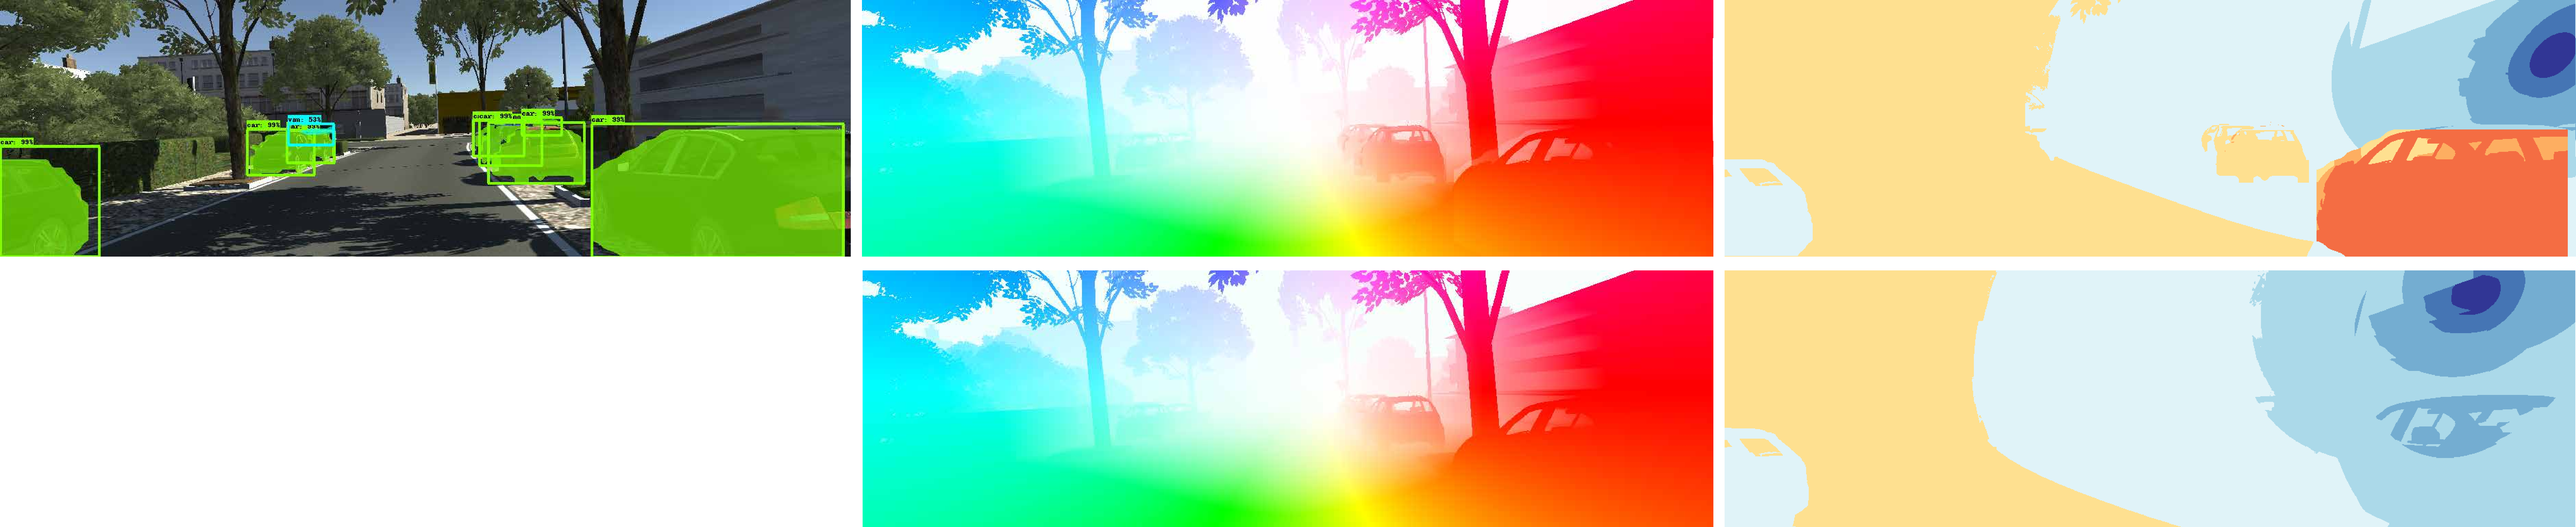
\includegraphics[width=\textwidth]{figures/moving}
\caption{
We visually compare a Motion R-CNN ResNet trained without (upper row) and
with (lower row) classifying the objects into moving and non-moving objects.
Note that in the selected example, all cars are parking, and thus the predicted
motion in the first row is an error.
From left to right, we show the input image with instance segmentation results as overlay,
the estimated flow, as well as the flow error map.
The flow error map depicts correct estimates ($\leq 3$ px or $\leq 5\%$ error) in blue and wrong estimates in red tones.
}
\label{figure:moving}
\end{figure}

{
\begin{table}[t]
\centering
\begin{tabular}{@{}*{10}{c}@{}}
\toprule
\multicolumn{1}{c}{Network} & \multicolumn{5}{c}{Instance Motion} & \multicolumn{2}{c}{Camera Motion} &\multicolumn{2}{c}{Flow Error} \\
  \cmidrule(lr){1-1}\cmidrule(lr){2-6}\cmidrule(l){7-8}\cmidrule(l){9-10}
FPN        & $E_{R} [deg]$ & $E_{t} [m]$ & $E_{p} [m] $ & $O_{pr}$ & $O_{rc}$  & $E_{R}^{cam} [deg]$ & $E_{t}^{cam} [m]$ & AEE   & Fl-all \\\midrule
-          & (0.279)       & (0.442)     & -            & -        & -           & (0.220)             & (0.684)           & -     &     -\%    \\\midrule
$\times$   & 0.301         & 0.237       & 3.331        & 0.790    & 0.916       & 0.087               & 0.053             & 11.17 & 24.91\%    \\
\checkmark & 0.293         & 0.210       & 1.958        & 0.844    & 0.914       & 0.169               & 0.050             & 8.29  & 45.22\%    \\
  \bottomrule
\end{tabular}

\caption {
Evaluation of different metrics on the Virtual KITTI validation set.
AEE: Average Endpoint Error; Fl-all: Ratio of pixels where flow estimate is
wrong by both $\geq 3$ pixels and $\geq 5\%$.
We compare network variants with and without FPN.
All metrics are averaged over all examples in the validation set.
Quantities in parentheses in the first row are the average ground truth values for the estimated
quantity. For example, we compare the error in camera angle, $E_{R}^{cam} [deg]$,
to the average rotation angle in the ground truth camera motions.
}
\label{table:vkitti}
\end{table}
}

For our initial experiments, we concatenate both RGB frames as
well as the XYZ coordinates for both frames as input to the networks.
We train both, the Motion R-CNN ResNet and ResNet-FPN variants and supervise
camera and instance motions with 3D motion ground truth.

In Figure \ref{figure:vkitti}, we visualize instance segmentation and optical flow
results on the Virtual KITTI validation set.
In Figure \ref{figure:moving}, we visually justify the addition of the classifier
that decides between a moving and still object.
In Table \ref{table:vkitti}, we compare the performance of different network variants
on the Virtual KITTI validation set.

\paragraph{Camera motion}
Both variants achieve a low error in predicted camera translation, relative to
the average ground truth camera translation. The camera rotation angle error
is still relatively high, compared to the small average ground truth camera rotation.
Although both variants use the exact same network for predicting the camera motion,
the FPN variant performs worse here, with the error in rotation angle twice as high.
One possible explanations that should be investigated in futher work is
that in the FPN variant, all blocks in the backbone are shared between the camera
motion branch and the feature pyramid. In the variant without FPN, the C$5$ and
C$6$ blocks are only used in the camera branch, and thus only experience weight
updates due to the camera motion loss. This could mean that the weight updates due
to the RoI head losses are detrimental to the camera motion estimation.
As a remedy, increasing the loss weighting of the camera motion loss may be
helpful.

\paragraph{Instance motion}
The object pivots are estimated with relatively (given that the scenes are in a realistic scale)
high precision in both variants, although the FPN variant is significantly more
precise, which we ascribe to the higher resolution features used in this variant.

The predicted 3D object translations and rotations still have a relatively high
error, compared to the average actual (ground truth) translations and rotations,
which may be due to implementation issues, a non-optimal network architecture,
or problems with the current 3D motion ground truth loss
(e.g., non-optimal weighting between the components of the motion loss, or between motion and classification losses).
Note that the relative error is higher for rotations, which is
also the case in the camera motion estimates.
The FPN variant is only slightly more accurate for these predictions, which again suggests
that there may still be issues with our loss design, loss weighting, or implementation, as one would expect the
FPN to yield more accurate motion estimates (as is the case for the pivot estimation).

\paragraph{Instance segmentation}
Looking at Figure \ref{figure:vkitti}, our instance segmentation results are in
some cases still lacking the accuracy seen in the Mask R-CNN Cityscapes \cite{MaskRCNN} results,
which is likely due to implementation details.

\label{sec:experiments}

\section{Conclusion}
\parindent 2em
\onehalfspacing

We have introduced an extension on top of region-based convolutional networks to enable object motion estimation
in parallel to instance segmentation.
\todo{complete}

\subsection{Future Work}
\paragraph{Predicting depth}
In most cases, we want to work with raw RGB sequences for which no depth is available.
To do so, we could integrate depth prediction into our network by branching off a
depth network from the backbone in parallel to the RPN, as in Figure \ref{}.
Although single-frame monocular depth prediction with deep networks was already done
to some level of success,
our two-frame input should allow the network to make use of epipolar
geometry for making a more reliable depth estimate, at least when the camera
is moving.

\paragraph{Training on real world data}
Due to the amount of supervision required by the different components of the network
and the complexity of the optimization problem,
we trained Motion R-CNN on the simple synthetic Virtual KITTI dataset for now.
A next step will be training on a more realistic dataset.
For this, we can first pre-train the RPN on an object detection dataset like
Cityscapes. As soon as the RPN works reliably, we could execute alternating
steps of training on, for example, Cityscapes and the KITTI stereo and optical flow datasets.
On KITTI stereo and flow, we could run the instance segmentation component in testing mode and only penalize
the motion losses (and depth prediction if added), as no instance segmentation ground truth exists.
On Cityscapes, we could continue train the instance segmentation components to
improve detection and masks and avoid forgetting instance segmentation.
As an alternative to this training scheme, we could investigate training on a pure
instance segmentation dataset with unsupervised warping-based proxy losses for the motion (and depth) prediction.

\label{sec:conclusion}

%%%%%%%%%%%%%%%%%%%%%%%%%%%%%%%%%%%%%%%%%%%%%%%%%%
% Bibliografie mit BibLaTeX
%
% Verwende keyword=meinbegriff, um nur die Einträge aus deiner .bib-Datei ausgeben zu lassen, die mit meinbegriff getaggt sind.
% Darf ein bestimmtes Keyword nicht enthalten sein, verwende notkeyword=meinbegriff.
\singlespacing
\printbibliography[title=Bibliography, heading=bibliography]
%\printbibliography[title=Literaturverzeichnis, heading=bibliography, keyword=meinbegriff]


\clearpage
%%%%%%%%%%%%%%%%%%%%%%%%%%%%%%%%%%%%%%%%%%%%%%%%%%
% Beginn des Anhangs
\appendix

%% \pagenumbering{Roman}
%% \setcounter{page}{\value{savedromanpagenumber}+1} % gespeicherte Seitenzahl vom Beginn des Dokuments aufrufen und damit weiterzählen

\clearpage

\end{document}
